% Definiciones y constantes de estilo
\include{Definiciones}
\usepackage{float} %Para obligar a las figuras a quedarse en un sitio

% Definiciones de comandos
\newcommand{\nombreautor}{Javier Benavides Caro}
\newcommand{\nombredirector}{Juan Manuel López Navarro}
\newcommand{\nombretrabajo}{Desarrollo y puesta en funcionamiento de un sistema de adquisición EEG con capacidades de procesado}
\newcommand{\nombretrabajocorto}{Prototipado de sistema de adquisición EEG}
\newcommand{\fecha}{\today}
\newcommand{\lugar}{Madrid}
\newcommand{\master}{Máster Universitario en Ingeniería de Telecomunicación}
% Descomentar si tu trabajo tiene un co-director
%\newcommand{\nombrecodirector}{TODO: Nombre del co-director}
% Descomentar si tu trabajo está asociado a un grupo de investigación
% \newcommand{\grupoInvestigacion}{TODO: Grupo de investigación}
\newcommand{\departamento}{Grupo de investigación en Intrumentación y Acústica Aplicada}
\newcommand{\facultad}{Escuela Técnica Superior de Ingenieros de Telecomunición}
\newcommand{\universidad}{Universidad Politécnica de Madrid}
\newcommand{\pieparizq}{\nombretrabajocorto}
\newcommand{\pieparcen}{\nombretrabajocorto}
\newcommand{\logoizq}{logo_politecnica}
\newcommand{\logoder}{escudo_teleco}
\newcommand{\correo}{j.bcaro@alumnos.upm.es; javierbenacaro@gmail.com}


% Glosario y acrónimos
%% Acrónimos

%TODO: Añadir aquí los acrónimos
% Ejemplo de acrónimo
\newacronym{FPGA}{FPGA}{Field-Programmable Gate Array}
\newacronym{PCB}{PCB}{Print Board Circuit}
\newacronym{EEG}{EEG}{Electroencefalografía}
\newacronym{ECG}{ECG}{Electrocardiograma}
\newacronym{SPS}{SPS}{Samples Per Second}
\newacronym{ADC}{ADC}{Analogic to Digital Converter}

% Glosario

%TODO: Añadir aquí las definiciones del glosario
% Ejemplo de glosario
\newglossaryentry{bitstream}{name={bitstream},description={En este contexto se refiere al binario que configura el Hardware de la FPGA}}

\addbibresource{src/Bibliografia}  
% Acrónimos

%TODO: Añadir aquí los acrónimos
% Ejemplo de acrónimo
\newacronym{FPGA}{FPGA}{Field-Programmable Gate Array}
\newacronym{PCB}{PCB}{Print Board Circuit}
\newacronym{EEG}{EEG}{Electroencefalografía}
\newacronym{ECG}{ECG}{Electrocardiograma}
\newacronym{SPS}{SPS}{Samples Per Second}
\newacronym{ADC}{ADC}{Analogic to Digital Converter}

% Glosario

%TODO: Añadir aquí las definiciones del glosario
% Ejemplo de glosario
\newglossaryentry{bitstream}{name={bitstream},description={En este contexto se refiere al binario que configura el Hardware de la FPGA}}
% Inicio del documento
\begin{document}

% Elección del idioma (español)
\selectlanguage{spanish}

%
% Portada
%
\pagenumbering{gobble}
\setcounter{page}{0}
%
% Portada
%

% Universidad, Facultad
\begin{titlepage}
\selectlanguage{spanish}

\begin{figure}[h]
	\begin{center}
		\includegraphics[scale=0.35]{\logoizq}
		\hspace{10cm}
		\includegraphics[scale=0.4]{\logoder}
	\end{center}	
\end{figure}

\begin{center}
\textbf{\begin{LARGE}
\textsc{\universidad} \\
\end{LARGE}}
\bigskip 
\begin{LARGE}
\textsc{\textbf{\facultad}} \\
\end{LARGE}
\end{center}


% Grado
\begin{center}
\begin{Large}
\textsc{\master}\\
\end{Large}
\end{center}

\bigskip
\bigskip
\bigskip
\bigskip

% Nombre del TFM
\begin{center}
\textbf{\begin{large}
\MakeUppercase{\nombretrabajo}\\
\end{large}}
\end{center}

% Nombre del autor
\vspace{\fill}
\begin{center}
	\begin{large}
		\textbf{Autor: \nombreautor}\\
		% Tutor
		\bigskip
		\textbf{Director: \nombredirector}\\
		% Ponente, si está definido en main.tex
		\ifcsname nombrecodirector\endcsname
		\bigskip
		\textbf{Co-director: \nombrecodirector}\\
		\fi
		
		\bigskip
		\bigskip
		\bigskip
		
		% Fecha
		\textbf{\lugar, \fecha}\\
	\end{large}

\end{center}
\end{titlepage}

% Primera página
\pagenumbering{Alph}
\thispagestyle{empty}
\par\vspace*{\fill}
\begin{flushleft}
\begin{scriptsize}
\end{scriptsize}\end{flushleft}
\newpage
\thispagestyle{empty}
\begin{center}

% Nombre del trabajo
\textbf{\begin{large}
\MakeUppercase{\nombretrabajo}\\*
\end{large}}
\vspace*{0.2cm}
\vspace{5cm}

% Nombre del autor y del tutor
\large Autor: \nombreautor \\*
\large Director: \nombredirector \\*
\ifcsname nombrecodirector\endcsname
\large Co-director: \nombrecodirector\\
\fi

\vfill

% Grupo de investigación, departamento, facultad, universidad y fecha
\ifcsname grupoInvestigacion\endcsname
\grupoInvestigacion \\
\fi
\departamento \\
\facultad \\
\universidad \\
\vspace{1cm}
\fecha \\

\clearpage

\end{center}
\normalsize

\hypersetup{pageanchor=true}

% Estilo de párrafo de los capítulos
\setlength{\parskip}{0.75em}
\renewcommand{\baselinestretch}{1.25}
% Interlineado simple
\spacing{1}

%
% Agradecimientos
%


\chapter*{Dedicatoria}

TODO: Dedicatoria.

Lorem ipsum dolor sit amet, consectetur adipiscing elit. Phasellus laoreet dolor at sodales porta. Morbi facilisis hendrerit lacus vel sollicitudin. Aenean eleifend urna metus, eget vestibulum libero dictum tincidunt. Curabitur quis ultrices lorem. Duis ultricies, eros eget condimentum pharetra, tellus eros lobortis nulla, vel mattis nibh dui et felis. Interdum et malesuada fames ac ante ipsum primis in faucibus. Nam non lorem et ligula condimentum molestie. Fusce quis dolor non metus suscipit commodo. Praesent vel pulvinar lectus. Nullam ac dui eget magna accumsan volutpat. Aliquam sed purus quis lorem dictum rutrum auctor eu enim. Pellentesque a urna ac ligula cursus lacinia. Aenean sodales justo massa, vel imperdiet justo imperdiet ut. Nulla euismod pulvinar arcu eu convallis. Vivamus a tempus nunc, et vulputate nulla.

Sed dapibus aliquam imperdiet. Vivamus est quam, fermentum vitae augue id, ultricies tincidunt massa. Praesent tincidunt ex sem, ut aliquet nulla imperdiet eu. Duis ac ultricies lorem. Aenean consequat ipsum nec arcu aliquam, sit amet interdum quam tempus. In justo odio, bibendum vel nulla nec, aliquet tristique justo. In vel metus ut libero suscipit ultricies.

Class aptent taciti sociosqu ad litora torquent per conubia nostra, per inceptos himenaeos. Proin urna elit, iaculis id quam at, pretium laoreet ipsum. Phasellus ultricies faucibus ex et eleifend. Quisque facilisis erat dolor, ac rhoncus erat convallis et. Aliquam semper eleifend imperdiet. Sed eros ipsum, sagittis in pellentesque vel, vestibulum a augue. Duis sapien mauris, fringilla a tortor ut, sollicitudin volutpat nunc. Pellentesque vestibulum vel arcu in molestie. Nullam fermentum dolor luctus metus efficitur pulvinar. Pellentesque risus enim, tempus id ullamcorper in, maximus id nisl. Cras rhoncus consequat augue eu gravida. Ut efficitur mauris vitae orci dignissim sagittis. Suspendisse vitae massa eget nunc bibendum interdum.
  
\chapter*{Agradecimientos}

TODO: Agradecimientos.

Lorem ipsum dolor sit amet, consectetur adipiscing elit. Phasellus laoreet dolor at sodales porta. Morbi facilisis hendrerit lacus vel sollicitudin. Aenean eleifend urna metus, eget vestibulum libero dictum tincidunt. Curabitur quis ultrices lorem. Duis ultricies, eros eget condimentum pharetra, tellus eros lobortis nulla, vel mattis nibh dui et felis. Interdum et malesuada fames ac ante ipsum primis in faucibus. Nam non lorem et ligula condimentum molestie. Fusce quis dolor non metus suscipit commodo. Praesent vel pulvinar lectus. Nullam ac dui eget magna accumsan volutpat. Aliquam sed purus quis lorem dictum rutrum auctor eu enim. Pellentesque a urna ac ligula cursus lacinia. Aenean sodales justo massa, vel imperdiet justo imperdiet ut. Nulla euismod pulvinar arcu eu convallis. Vivamus a tempus nunc, et vulputate nulla.

Sed dapibus aliquam imperdiet. Vivamus est quam, fermentum vitae augue id, ultricies tincidunt massa. Praesent tincidunt ex sem, ut aliquet nulla imperdiet eu. Duis ac ultricies lorem. Aenean consequat ipsum nec arcu aliquam, sit amet interdum quam tempus. In justo odio, bibendum vel nulla nec, aliquet tristique justo. In vel metus ut libero suscipit ultricies.

Class aptent taciti sociosqu ad litora torquent per conubia nostra, per inceptos himenaeos. Proin urna elit, iaculis id quam at, pretium laoreet ipsum. Phasellus ultricies faucibus ex et eleifend. Quisque facilisis erat dolor, ac rhoncus erat convallis et. Aliquam semper eleifend imperdiet. Sed eros ipsum, sagittis in pellentesque vel, vestibulum a augue. Duis sapien mauris, fringilla a tortor ut, sollicitudin volutpat nunc. Pellentesque vestibulum vel arcu in molestie. Nullam fermentum dolor luctus metus efficitur pulvinar. Pellentesque risus enim, tempus id ullamcorper in, maximus id nisl. Cras rhoncus consequat augue eu gravida. Ut efficitur mauris vitae orci dignissim sagittis. Suspendisse vitae massa eget nunc bibendum interdum.
  

%
% Resumen
%
\pagenumbering{roman}
\setcounter{page}{0}
% Resumen en español
\chapter*{Resumen}

\begin{abstractEs}

Este proyecto tiene como objetivo el diseño y prototipado de un sistema de adquisición y procesado de electroencefalogramas. 
El sistema desarrollado cuenta con un microcontrolador de la familia ARM Cortex M4 como núcleo de procesamiento y gestión de dispositivos. Este microcontrolador se encargará de la configuración y comunicación con el ADC (ADS1299), chip que realiza la adquisición de los datos que conforman el electroencefalograma. Además, el ARM procesará y filtrará la información obtenida.
Finalmente se transmitirá esta información a un ordenador utilizando una de las dos interfaces inalámbricas disponibles (WiFi). Se ha realizado un software para el ordenador que permite cambiar la configuración del sistema de adquisición y representar los datos procesados en gráficas.
	
\end{abstractEs}

% Palabras clave en español
\begin{keywordsEs}
	ADC, adquisición, filtrado, microcontrolador, PCB, interfaz.
\end{keywordsEs}


% Resumen en inglés
\chapter*{Abstract}

\begin{abstractEn}

The objective of this project is the design and prototyping of an electroencephalogram acquisition and processing system.
The developed system has a microcontroller of the ARM Cortex M4 family as the core of processing and device management. This microcontroller will be responsible for the configuration and communication with the ADC (ADS1299), chip that performs the acquisition of the data that conforms the electroencephalogram. In addition, the ARM will process and filter the information obtained.
Eventually this information will be transmitted to a computer using one of the two available wireless interfaces (WiFi). A user interface created using LabView will be able to change the configuration and represent all the adquired data.

\end{abstractEn}

% Palabras clave en inglés
\begin{keywordsEn}
ADC, adquisition, filtering, microcontroller, PCB, interface.
\end{keywordsEn}




%
% Glosario
%
% Para que aparezca al comienzo del documento será necesario compilar con una copia de ambas sentencias al final 2 veces.  Tras comprobar que aparece en el final eliminar esas sentencias y debería cargar el glosario aquí
%\printglossary[type=\acronymtype]
%\printglossary


% Estilo de párrafo de los índices
\setlength{\parskip}{1pt}
\renewcommand{\baselinestretch}{1}

%
% Tabla de contenidos
%
\tableofcontents
\listoffigures
\listoftables
\cleardoublepage

% Estilo de párrafo de los capítulos
\setlength{\parskip}{0.75em}
\renewcommand{\baselinestretch}{1.25}
% Interlineado simple
\spacing{1}
% Numeración contenido
\pagenumbering{arabic}
\setcounter{page}{1}

%
% Introducción
%
\chapter{Introducción\label{sec:introduccion}}

Desde el principio de los tiempos la humanidad se ha esforzado por comprender el entorno que le rodea, aprender de él y usarlo en su propio beneficio para conseguir así hacer su vida más fácil. Por el momento hemos conseguido hacer volar aviones gracias a la observación de los pájaros o crear sistemas de sonar que se asemejan al sistema que utilizan los murciélagos para orientarse. Pero irónicamente, a pesar del esfuerzo invertido, nuestro propio cuerpo sigue albergando secretos que desentrañar que podrían facilitarle la vida a un gran número de personas.

El estudio del cuerpo humano ha sido uno de los temas más polémicos y que más ha evolucionado desde que hay registro. Aunque al comienzo estuvo muy marcado por la superstición y la religión, achacando la mayoría de las dolencias y efectos científicos a la magia, con el paso del tiempo aparecieron personas como Hipócrates y Aristóteles que fueron capaces de aportar un nuevo enfoque basado en la observación y estudio de lo que les rodeaba, asentando unas bases que, posteriormente, serían aprovechadas y mejoradas hasta convertirse en lo que conocemos hoy en día como método científico.

El estudio del cuerpo humano ha seguido diferentes fases a lo largo de la historia. Comparar el cuerpo humano con animales fue uno de los primeros pasos para descubrir cómo estábamos formados por dentro. Posteriormente, aprovechando los cuerpos de personas ya fallecidas se estudió la anatomía humana, permitiendo así crear mapas y dibujos de la estructura del cuerpo humano y sus órganos bastante detallados.

\begin{figure} [H]
    \centering
    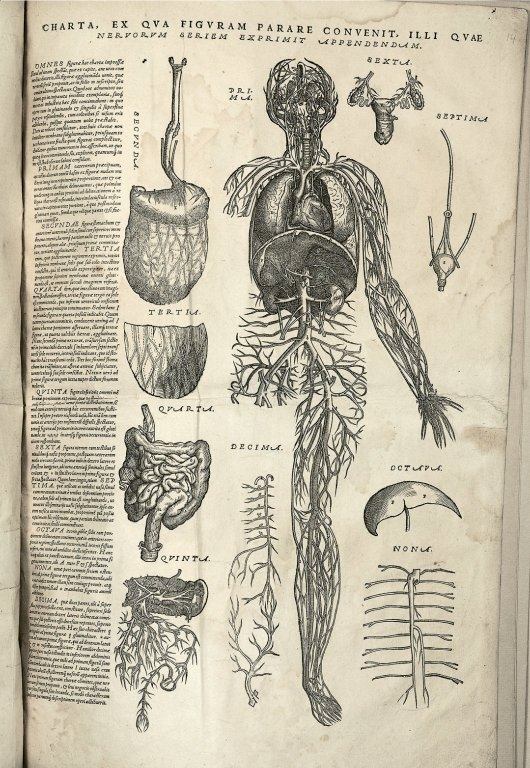
\includegraphics[width=0.25\textwidth]{Anatomia}
    \caption{Ejemplo de anatomía humana.}
    \label{fig:Anatomia}
\end{figure}

Pese a todo, estudiar cuerpos inertes tiene sus limitaciones de modo que durante un tiempo se realizaron vivisecciones para poder comprender mejor como funcionaban todos aquellos órganos, músculos y nervios que ya habían visto con anterioridad. Con el paso del tiempo este sistema fue descartado ya que es una práctica que ponía en peligro la vida del sujeto, haciéndolo pasar por una experiencia terrible en el mejor de los casos.

En la actualidad, gracias al conocimiento acumulado de muchos años y a los avances en otros campos de la ciencia, se han desarrollado dispositivos y técnicas que permiten el estudio en vivo del comportamiento del cuerpo humano de forma no invasiva. Es posible utilizar ecografías para ver el estado del corazón, radiografías para diagnosticar un hueso roto e incluso técnicas más avanzadas como la medicina nuclear que permiten saber que partes del cerebro se activan frente a determinados estímulos sin necesidad de interactuar físicamente con él.

Si bien todas las técnicas anteriores han supuesto auténticos hitos en la medicina moderna y han permitido diagnosticar un gran número de enfermedades así como mejorar la calidad de vida de muchas personas, la mayoría presenta inconvenientes que hacen improbable su uso a nivel personal o docente debido al tamaño de los equipos necesarios para su realización o el coste muy elevado del procedimiento (sin contar con el conocimiento necesario para la realización correcta de la prueba).

Teniendo en mente esta problemática se han desarrollado dispositivos capaces de medir pequeñas las variaciones de voltaje que se producen en el interior de nuestro cuerpo haciendo uso de unos dispositivos denominados electrodos.
\\De esta forma es posible, con un coste muy reducido y un equipamiento relativamente asequible, conseguir inferir que procesos químicos y físicos se están produciendo en el interior de nuestro cuerpo.

Haciendo uso de este sistema y en función del origen de dichas señales dichos registros reciben distintos nombres: electrocardiograma (ECG) para las señales originadas por las contracciones del corazón; electromiograma (EMG) para las generadas en los músculos; electroencefalograma (EEG) para aquellas generadas en el cerebro, etc.

\begin{figure} [H] %this figure will be at the center
    \centering
    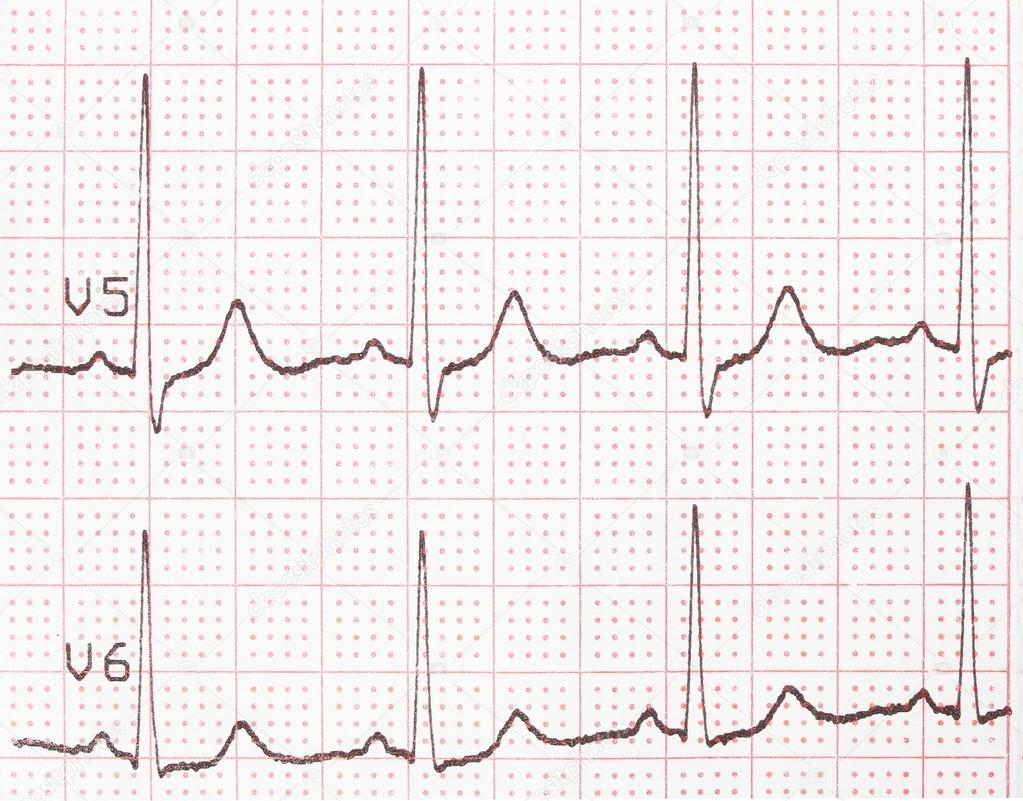
\includegraphics[width=7.5cm]{ECG}
    \caption{Ejemplo de ECG}
    \label{fig:ECG}
\end{figure}

\section{Alcance y estructura del proyecto}
El objetivo de este proyecto es realizar un sistema capaz de captar señales de electroencefalogramas (EEG) manteniendo una buena relación prestaciones/coste. El sistema estará compuesto de dos tarjetas, una de acondicionamiento y de adquisición de datos basada en el circuito integrado ADS1299 y otra de procesamiento y transmisión de dicha información. Esta última es el objetivo del presente proyecto. La plataforma de procesamiento estará basada en un procesador de altas prestaciones, dispondrá de interfaces Wifi, Bluetooth y almacenamiento USB para la transmisión y almacenamiento de los datos respectivamente. 

En la primera fase del proyecto se seleccionará el microcontrolador más adecuado entre los existentes en el mercado analizando características como: capacidad de procesado, interoperación con otros dispositivos, prestaciones...
\\Se compararán los microcontroladores ofrecidos por los distintos fabricantes (ST Microelectronics, Texas instruments, etc) y finalmente, se escogerá aquel que mejor se adecúe a las necesidades del proyecto siendo los principales candidatos los de la familia ARM-M4 STM32F4x por su excelente relación prestaciones-coste.
\\Se valorará también la posibilidad de utilizar diferentes herramientas para la programación del microcontrolador y las alternativas open source en caso de existir.

Una vez hecho el diseño eléctrico de la tarjeta se procederá al diseño de una PCB, la cual se implementará utilizando tecnología SMD en su mayor parte. Para el diseño de la placa se utilizará KiCad por las numerosas ventajas que presenta al ser software libre y la gran cantidad de información que se puede encontrar sobre el funcionamiento del mismo.
Tras depurar la PCB, se implementará un sencillo firmware que permita testear el hardware diseñado y hacer una adquisición básica utilizando la tarjeta SAD utilizando los distintos interfaces implementados.

Adicionalmente se pondrá en marcha un programa para el ordenador basado en LabView donde presentar los datos recibidos.

\section{Base teórica\label{sec:Base_teorica}}

% Documentación interesante para esta sección: 
% http://slideplayer.es/slide/3413933/

Antes de empezar a desarrollar el dispositivo ya mencionado es indispensable realizar una investigación previa del origen de las señales que se quieren adquirir, haciendo especial hincapié en las características de las mismas.

\begin{wrapfigure}[14]{R}{8cm}
    \centering
    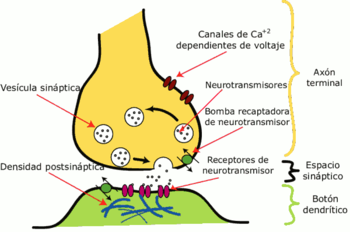
\includegraphics[width=8cm]{Intro_neuronas}
    \caption{Sinapsis neuronal \cite{wikipedia}}
    \label{fig:Intro_neuronas}

\end{wrapfigure}
En el cerebro se realizan \textbf{millones de conexiones} diarias entre las células que la conforman. Dichas células reciben el nombre de \textbf{neuronas}. La comunicación entre ellas se realiza mediante el \textbf{intercambio de neurotransmisores}, proceso que recibe el nombre de sinapsis y que provoca una corriente eléctrica de mayor o menor intensidad que permite la inhibición o activación de las distintas neuronas. 

La suma de todas las corrientes eléctricas conforma lo que se denomina \textbf{actividad bioeléctrica cerebral}. Mediante el uso de sensores es posible medirla y representarla.

Las señales del \acrshort{EEG} dependen del estado de consciencia del usuario y se pueden clasificar en función de su amplitud y frecuencia. Las principales ondas son las siguientes\footnote{Contenido obtenido de \cite{apuntes}}:

\begin{itemize}
\item\textbf{Ondas delta} (hasta 3.5 Hz). Término introducido por W. G. Walter en 1937 para describir a estas ondas de baja frecuencia y alta intensidad (unos centenares de $\mu$V). Tienen lugar en niños de corta edad y en adultos sólo en estado de sueño profundo, inconsciencia o situaciones que aumenten la presión intercraneal como tumores cerebrales.
\end{itemize}
\begin{figure} [H]
    \centering
    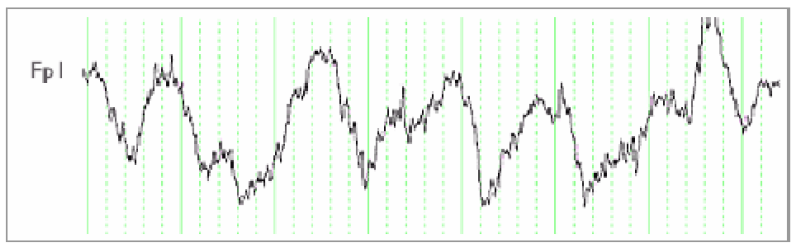
\includegraphics[width=13cm]{ondas_delta}
    \caption{Ondas delta \cite{apuntes}}
    \label{fig:ondas_delta}
\end{figure}

\clearpage

\begin{itemize}
\item\textbf{Ondas theta} (3.5 - 7.5 Hz). Término también Walter aunque mucho más tarde, en 1953. Estas ondas de amplitud inferior a 20 $\mu$ se dan durante el proceso de maduración en toda la corteza cerebral, aunque predomina en la región occipital y temporal y es más rápida en la zona frontal. Dominante en niños entre 5 y 7 años y aún quedan rastros en la juventud. En adultos y adolescentes se asocia a situaciones emocionales y pensamientos de tipo creativo, a estrés o a desordenes psíquicos.
\end{itemize}
\begin{figure} [H]
    \centering
    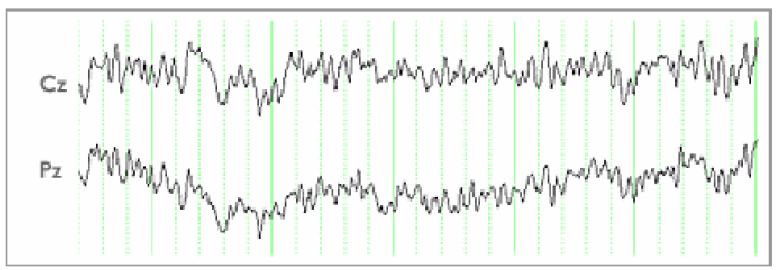
\includegraphics[width=13cm]{ondas_theta}
    \caption{Ondas theta \cite{apuntes}}
    \label{fig:ondas_theta}
\end{figure}

\begin{itemize}
\item\textbf{Ondas alfa} (7.5 - 12.5 Hz). Berger utilizó el término de ritmo alfa para ráfagas de 20-100 $\mu$V de amplitud y gran periodicidad a esas frecuencias predominantes sobre la región occipital pero que aparecen en todo el córtex. Se asocian a estados de relajación, de inactividad y son muy patentes en ausencia de estímulos visuales. Existe mucha variabilidad interpersonal en el ritmo alfa.
\end{itemize}
\begin{figure} [H]
    \centering
    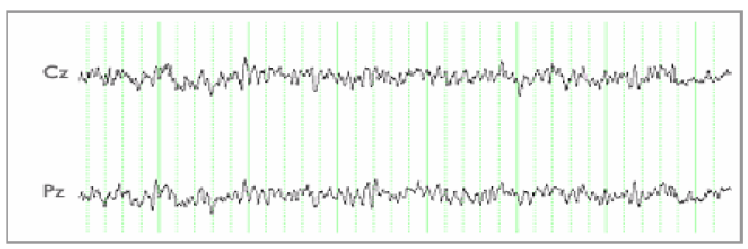
\includegraphics[width=13cm]{ondas_alfa}
    \caption{Ondas alfa \cite{apuntes}}
    \label{fig:ondas_alfa}
\end{figure}

\begin{itemize}
\item\textbf{Ondas beta} (12.5 - 30 Hz). Estas señales de pequeña amplitud, por debajo de 20$\mu$V, son bastante comunes y predominan durante la edad adulta. Suele dividirse en beta baja, beta media y beta alta. El ritmo beta bajo se suele localizar en los lóbulos frontal y occipital y los otros dos están menos localizados. Más irregular que el ritmo alfa, se asocia a actividad psicofísica, estados de agitación, alerta o la actividad mental que se realiza en la resolución de problemas.
\end{itemize}
\begin{figure} [H]
    \centering
    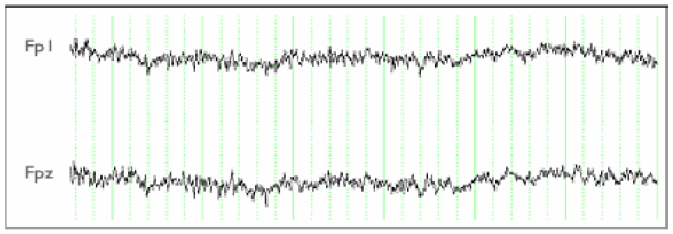
\includegraphics[width=13cm]{ondas_beta}
    \caption{Ondas beta \cite{apuntes}}
    \label{fig:ondas_beta}
\end{figure}

\begin{itemize}
\item\textbf{Ondas gamma} (12.5 - 30 Hz). Esta banda tiene un pico de resonancia, similar a los ritmos alfa, cercano a 40Hz al que se da el nombre de épsilon que se asocia a actividad mental abstracta que interviene en percibir como único por ejemplo el olor, los rasgos de la cara, la personalidad y la voz de una persona. Actualmente hay quien habla de ondas de frecuencias superiores a 50 Hz, son las hipergamma hasta 100 Hz y las lambda hasta 200 Hz, se dice aparecen en los monjes tibetanos en estados de meditación profunda
\end{itemize}

Para la realización de un electroencefalograma existe una disposición estándar en la colocación de los sensores denominada \textbf{sistema 10-20}. Se trata de un sistema internacional que indica la posición en la que se deben colocar los electrodos para una medición del \acrshort{EEG}.  Este sistema separa el cuero cabelludo en torno a un eje Z, colocando los electrodos numerado de manera par a la derecha y los impares a la izquierda (tal y como se puede ver en la figura \ref{fig:colocacion_electrodos)}.

\begin{figure} [H]
    \centering
    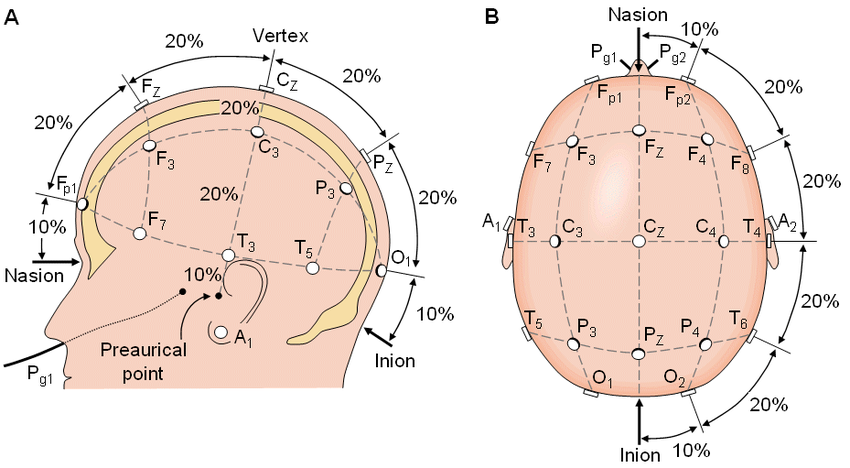
\includegraphics[width=12cm]{colocacion_electrodos}
    \caption{Esquema de colocación de los electrodos}
    \label{fig:colocacion_electrodos}
\end{figure}

\clearpage

\section{Tipos de electrodos\label{sec:Tipos_Electrodos}}

Los electrodos hacen la función de interfaz adaptadora entre los distintos medios por los que se transmiten las señales permitiendo así obtener una señal de mejores características. Este es un funcionamiento similar al de los huesos del oído, pues estos adaptan la señal acústica para que la señal percibida en la coclea tenga unas características determinadas. El funcionamiento de la mayoría de los dispositivos de adquisición de señales en el cuerpo humano depende de estos elementos y hacen uso de dos tipos principales, de trabajo y auxiliar.
\\El electrodo denominado ``de trabajo'' (\textit{working electrode}) es el que adquiere la señal de interés. El otro, denominado auxiliar, es el encargado de crear una referencia. El esquema de la figura \ref{fig:electrodos} muestra un esquema básico de funcionamiento:

\begin{figure} [h]
    \centering
    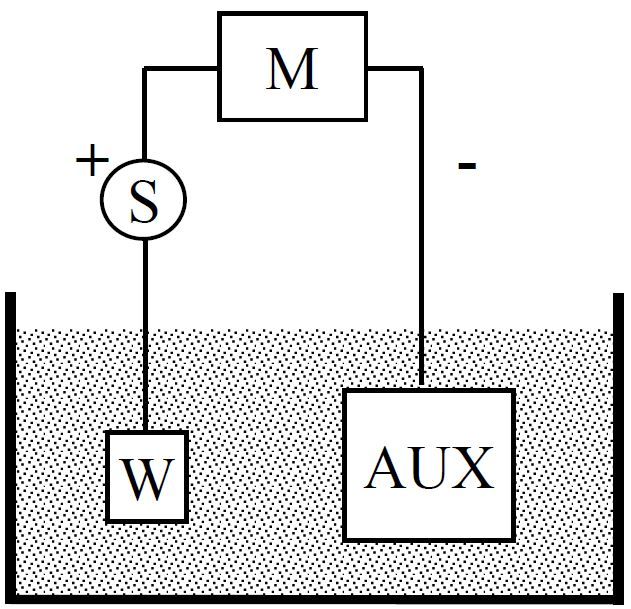
\includegraphics[width=7cm]{electrodos}
    \caption{Electrodos de en un sistema de adquisición \cite{apuntes}}
    \label{fig:electrodos}
\end{figure}

En función del método utilizado por el electrodo para hacer la interfaz con el cuerpo humano estos electrodos se pueden dividir en dos grandes grupos, cada uno con sus ventajas e inconvenientes. 

\subsection{Electrodos húmedos\label{sec:Elec_humedos}}

Los electrodos húmedos se caracterizan por utilizar algún material acuoso para realizar la interfaz entre el dispositivo y el cuerpo humano. Al estar conformados por varios materiales de distinta naturaleza estos electrodos suelen ser de construcción compleja. La figura \ref{fig:electrodo_humedo_2} muestra el esquema de un electrodo húmedo.

\begin{figure} [H]
    \centering
    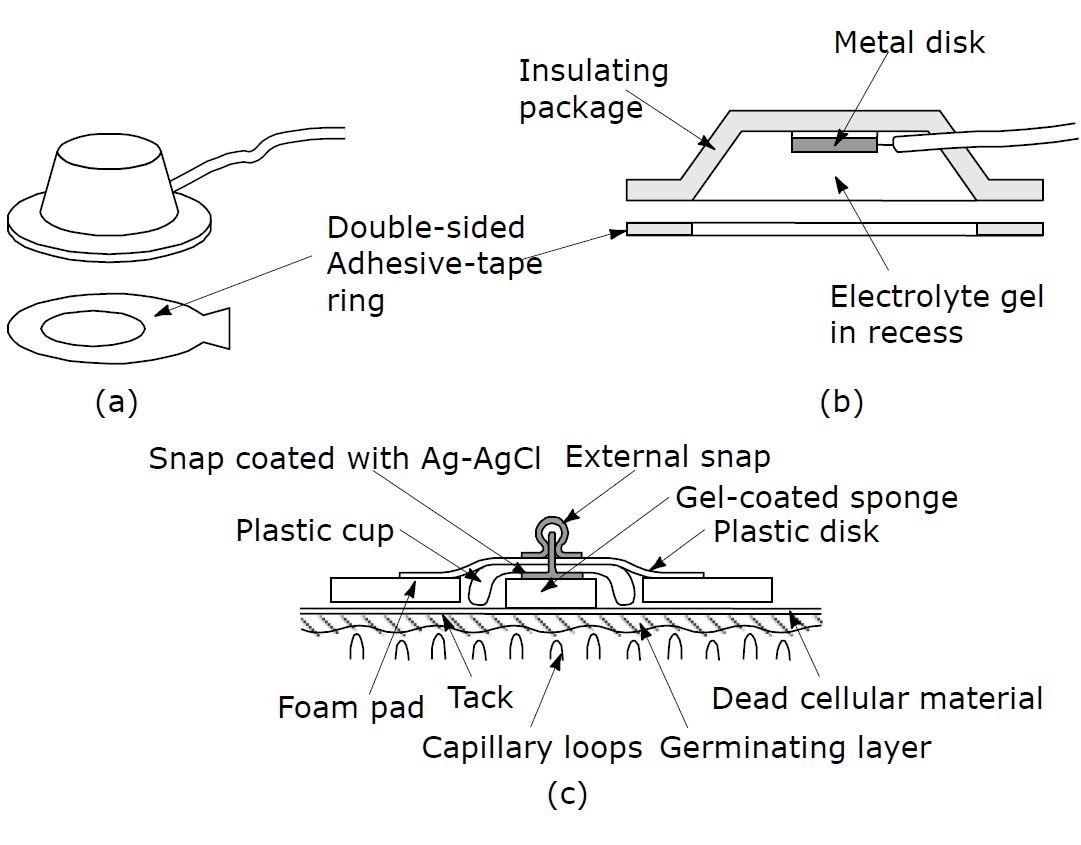
\includegraphics[width=10cm]{electrodo_humedo_2}
    \caption{Esquema de un electrodo húmedo \cite{apuntes}}
    \label{fig:electrodo_humedo_2}
\end{figure}

Estos dispositivos suelen dar muy buen resultado, consiguiendo señales con una buena amplitud y \acrshort{SNR} pero el material utilizado como interfaz suele ser desechable lo que obliga a usar electrodos de usar y tirar o a tener que dedicar mucho tiempo en la preparación y rellenado con gel de la cámara interior del dispositivo. Además, desde el punto de vista de la comodidad del usuario, la utilización de electrodos húmedos puede resultar incómoda al obligarlo a lavar la zona antes y después de su utilización.

La figura \ref{fig:electrodo_humedo_1} muestra un ejemplo de adquisición de \acrshort{EEG} utilizando electrodos húmedos.

\begin{figure} [h]
    \centering
    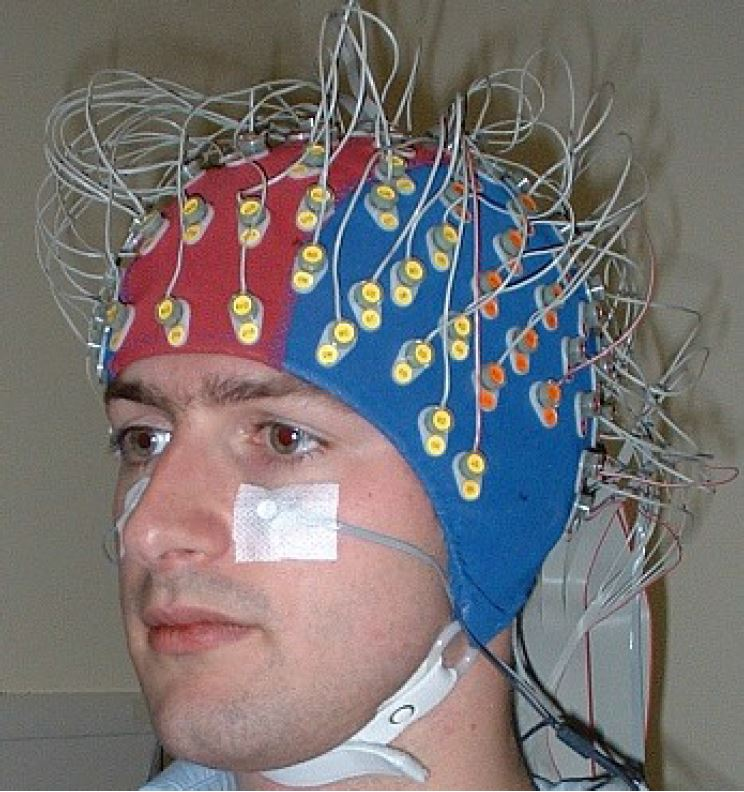
\includegraphics[width=7cm]{electrodo_humedo_1}
    \caption{Medida de un EEG usando electrodos húmedos \cite{apuntes}}
    \label{fig:electrodo_humedo_1}
\end{figure}

\clearpage

\subsection{Electrodos secos\label{sec:Elec_secos}}

Los electrodos secos utilizan materiales sólidos cuya interacción con el cuerpo humano resulta favorable. Al realizar una interfaz con materiales sólidos las señales se transmiten con mayor dificultad, pero este sistema resulta mucho más cómodo para el usuario y los electrodos son de fabricación más sencilla y reutilizables. La figura \ref{fig:electrodo_seco} muestra una representación 3D de un electrodo seco (derecha) y un electrodo seco real junto con sus correspondientes conectores (izquierda).

\begin{figure} [h]
    \centering
    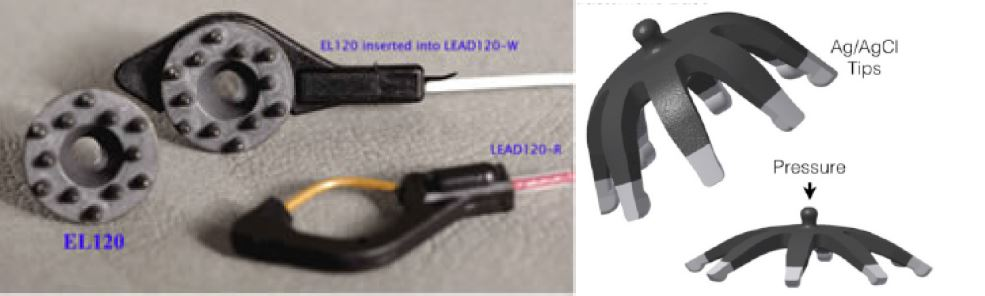
\includegraphics[width=13cm]{electrodo_seco}
    \caption{Electrodo seco real(izquierda) y representación 3D (derecha) \cite{apuntes}}
    \label{fig:electrodo_seco}
\end{figure}

Por comodidad durante la realización de este proyecto se utilizarán principalmente electrodos secos pero la posibilidad de usar electrodos húmedos se mantendrá, pues la utilización de unos u otros afecta al usuario final y a los resultados pero apenas al equipo encargado de su adquisición.

%
% Estado del arte
%
\chapter{Estado del Arte\label{sec:EstadoDelArte}}

Con el paso del tiempo se ha demostrado que una de nuestras mayores virtudes como seres humanos es la habilidad de aprovechar el saber cultivado por otras personas para realizar nuevos descubrimientos con mayor facilidad. En la actualidad con la ayuda de Internet esta ventaja se ha visto potenciada hasta límites insospechados.

Como se ha mencionado con anterioridad en el capítulo \ref{sec:introduccion}, a lo largo de los años se han desarrollado numerosas alternativas a los dispositivos presentes en los hospitales y laboratorios utilizados normalmente para el estudio del cerebro. 
\\Aunque se han invertido muchos recursos en estos dispositivos, el objetivo es permitir ampliar el número de personas capaces de estudiar el cerebro humano, consiguiendo  así aumentar las posibilidades de mejorar nuestro conocimiento sobre el mismo.

De esta forma debería ser más fácil realizar nuevos descubrimientos como, por ejemplo, encontrar nuevas formas de diagnosticar enfermedades o de realizar una comunicación hombre-máquina para aquellas personas que por un motivo u otro no pueden utilizar los medios convencionales.

A lo largo de este capítulo se presentarán algunos de los dispositivos capaces de capturar un EEG haciendo uso de electrodos, algunos a nivel personal, otros enfocados a la docencia y, por supuesto, algunos diseñados por empresas con el fin de realizar un producto final.


Historia procesadores (Gráfica de procesadores)
Antecedentes de la placa (Open BCI)

%
% Diseño
%
\chapter{Diseño\label{sec:diseño}}

Este proyecto consiste en una ampliación y cambio de enfoque de otro proyecto llevado a cabo de manera simultánea por una alumna de la Universidad Politécnica de Madrid llamada Nerea Urrestarazu que a su vez se basa en el Kit de demostración de rendimiento del ADS1299 proporcionado por Texas Instrument.

\begin{figure} [h]
    \centering
    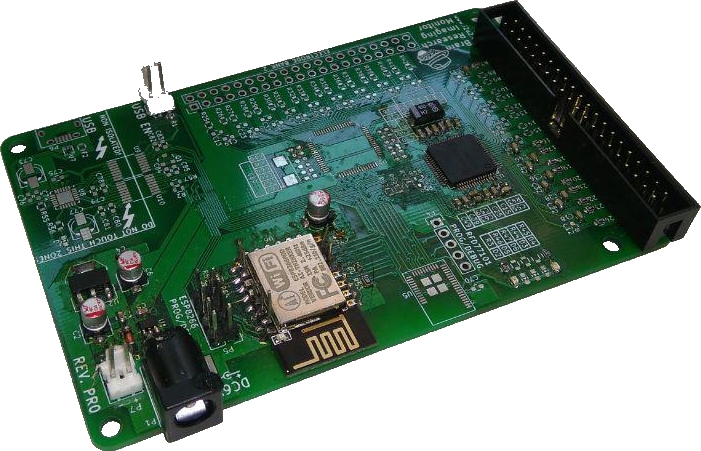
\includegraphics[width=7cm]{Placa_Nerea}
    \caption{Placa final del proyecto base}
    \label{fig:Placa_base}
\end{figure}

\section{Diseño base\label{sec:Diseno_base_N}}

El proyecto original trata sobre el diseño y desarrollo de una placa de adquisición de EEG haciendo uso de los integrados ADS1299 junto con un sistema de transmisión hacia el ordenador tanto inalámbricamente como a través de USB. La figura \ref{fig:Diseno_base} muestra las partes que componen dicho diseño.

\begin{figure} [h]
    \centering
    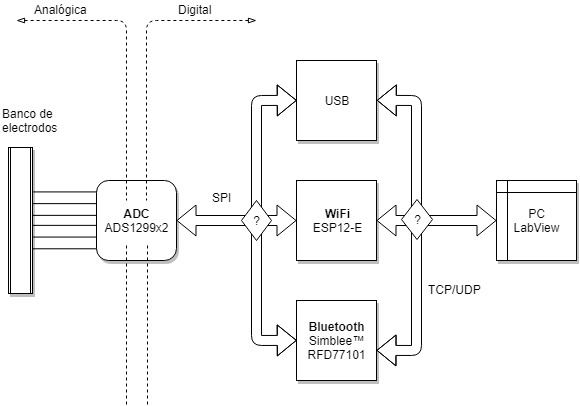
\includegraphics[width=12cm]{Esquema_diseno_base}
    \caption{Esquema del proyecto base}
    \label{fig:Diseno_base}
\end{figure}

\subsection{Adquisición de datos\label{sec:Adquisicion_N}}

La parte encargada de la adquisición está compuesta por un par de bancos de electrodos dispuestos en los laterales de la placa seguidos de un filtro paso-bajo con frecuencia de corte de 6.79kHz encargado de eliminar las componentes de frecuencias muy altas, no deseadas en el estudio de un \acrshort{EEG}. A continuación se encuentran conectados a sus respectivos bancos los \acrshort{ADC} ADS1299. 
\\Estos convertidores son capaces de adquirir información de forma independiente o en modo ``Daisy Chain'' y transmitirla a través de \acrshort{SPI} hacia otros dispositivos cuya misión será gestionarla.

\begin{figure} [h]
    \centering
    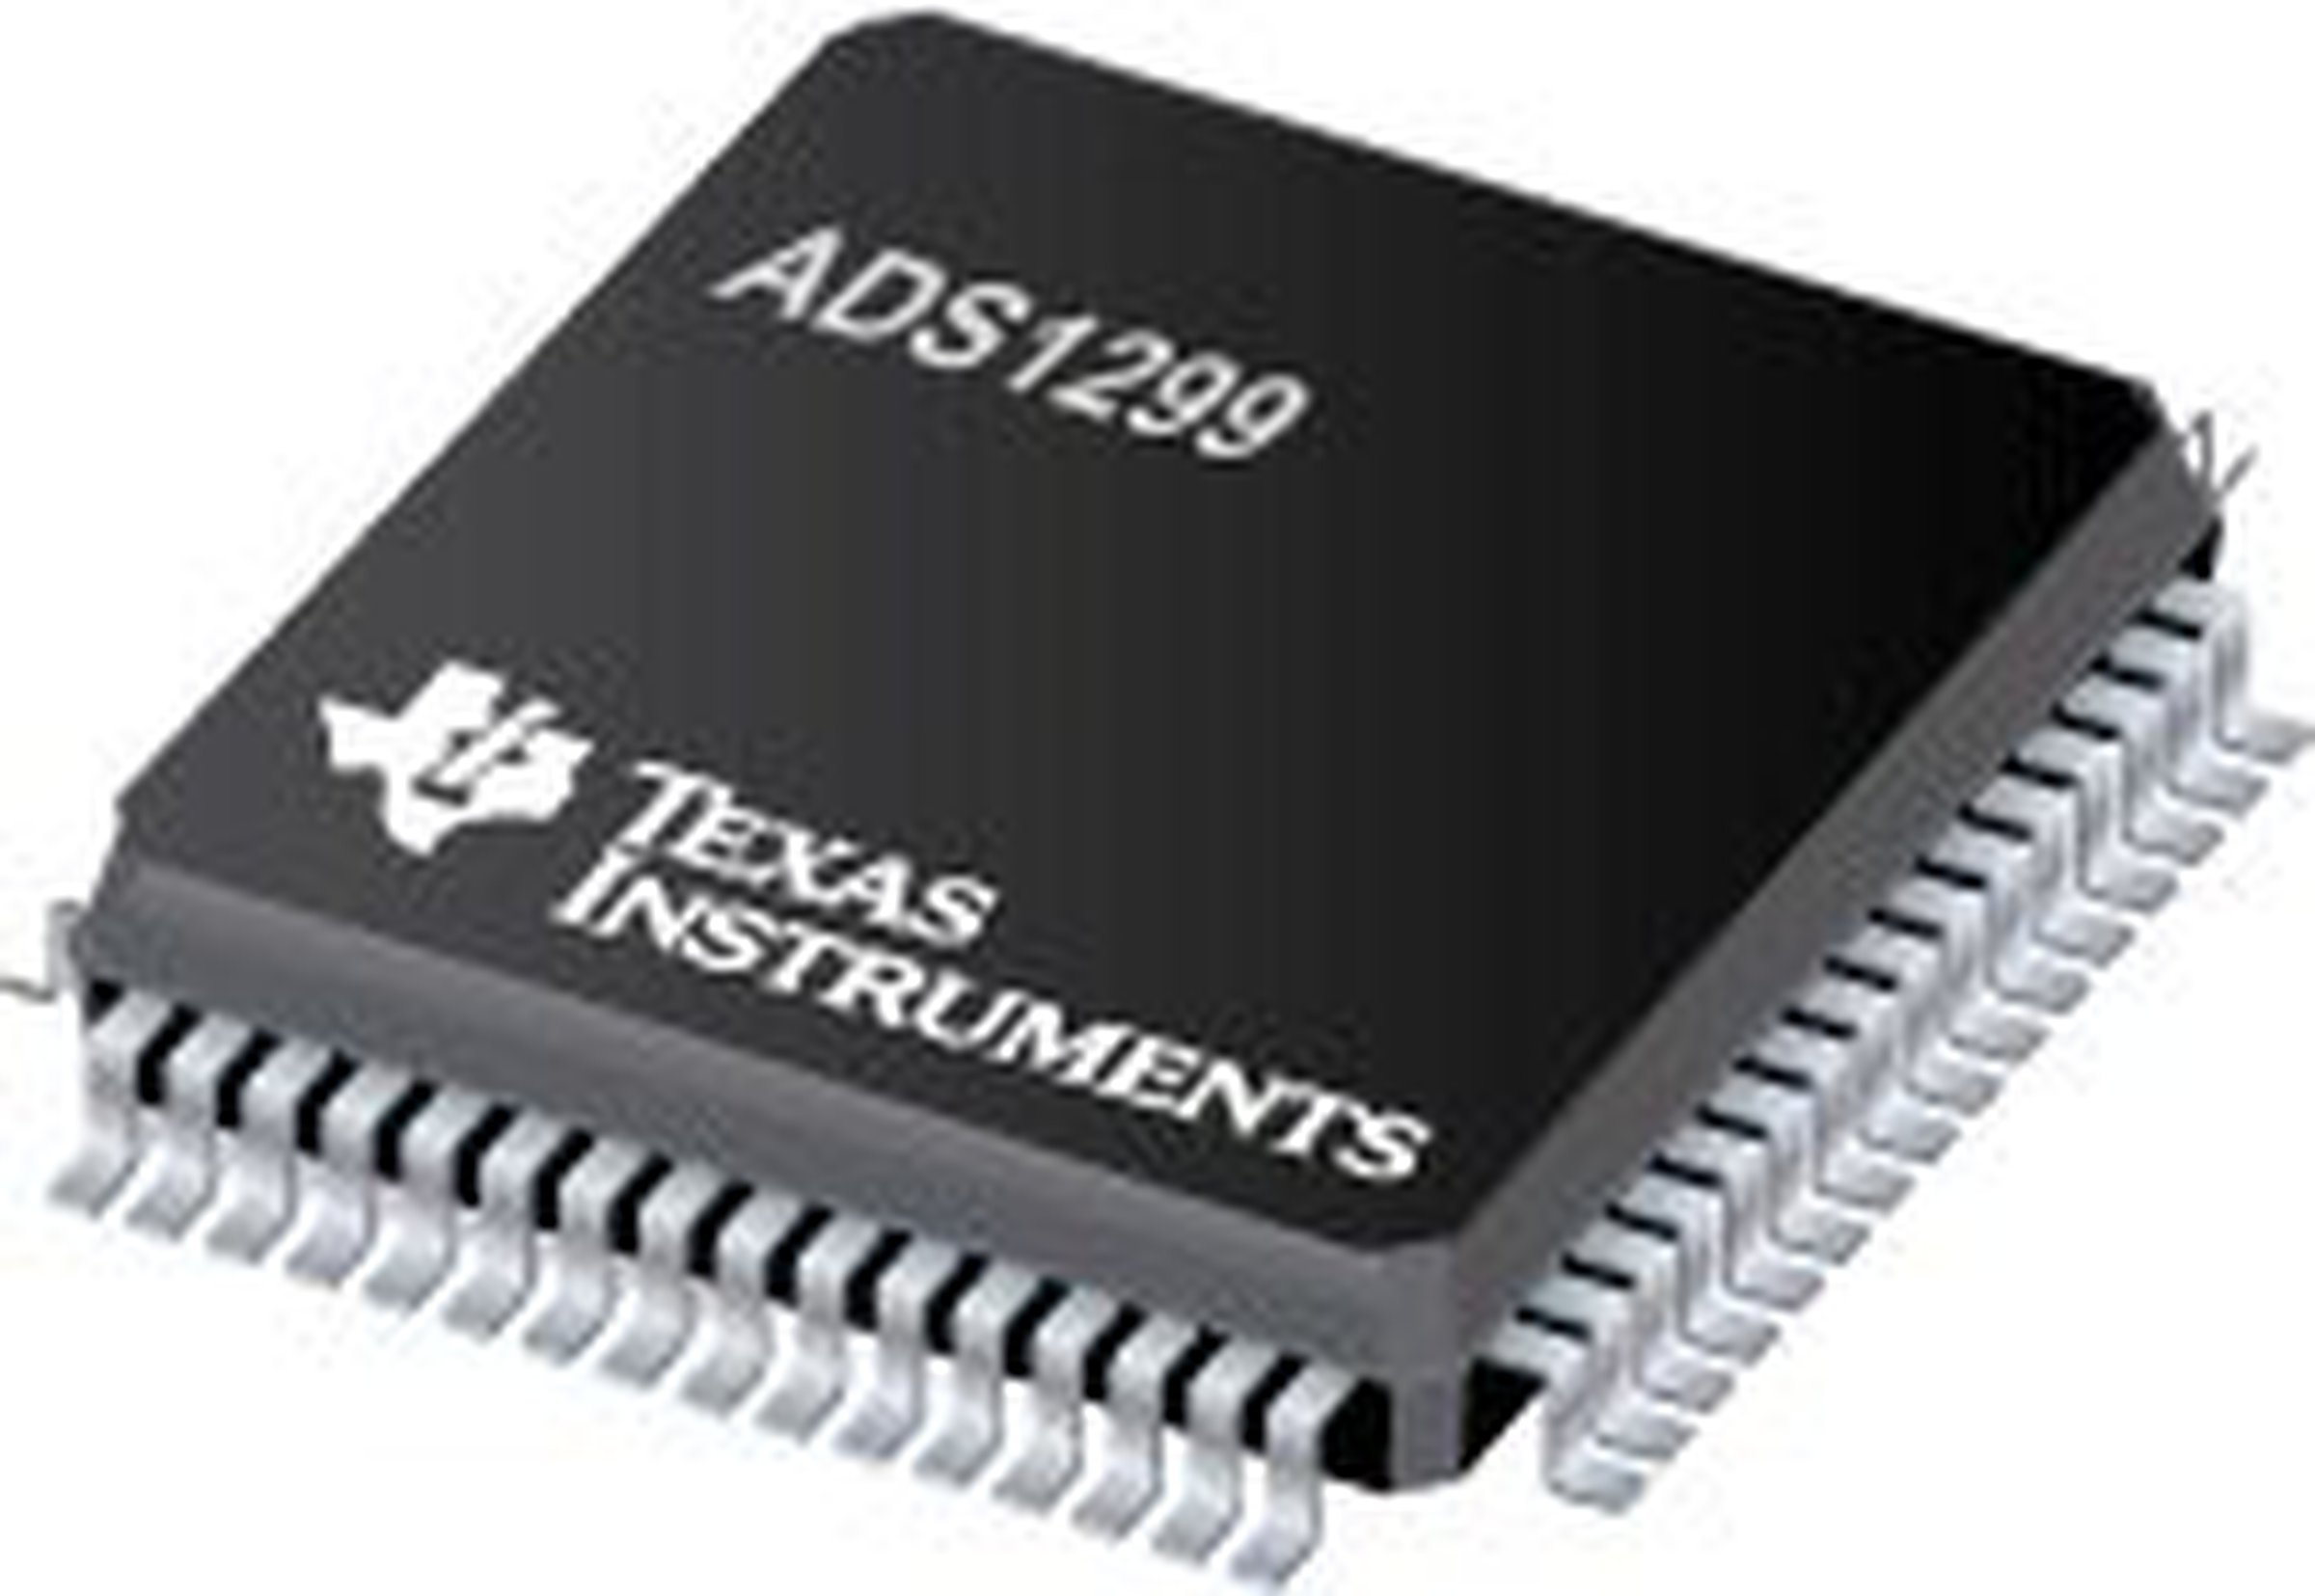
\includegraphics[width=6cm]{ADS1299}
    \caption{Convertidor Analógico-Digital ADS1299}
    \label{fig:ADS1299}
\end{figure}

El \acrshort{SPI} presente en el convertidor permite leer todos los registros del ADS y escribir la gran mayoría. Aunque normalmente se leen los relacionados con los datos convertidos, también es posible saber el estado de los \acrshort{GPIO} o el identificador único del dispositivo leyendo su registro asociado.

La configuración del ADS se realiza mediante la escritura de ciertos registros, cada uno asociado a un parámetro específico. La tabla \ref{tab:Conf_Reg_ADS} muestra los registros disponibles, tanto de lectura como de configuración, una descripción básica y la dirección de memoria asociada a los mismos.

\begin{table} [h]
    \centering
    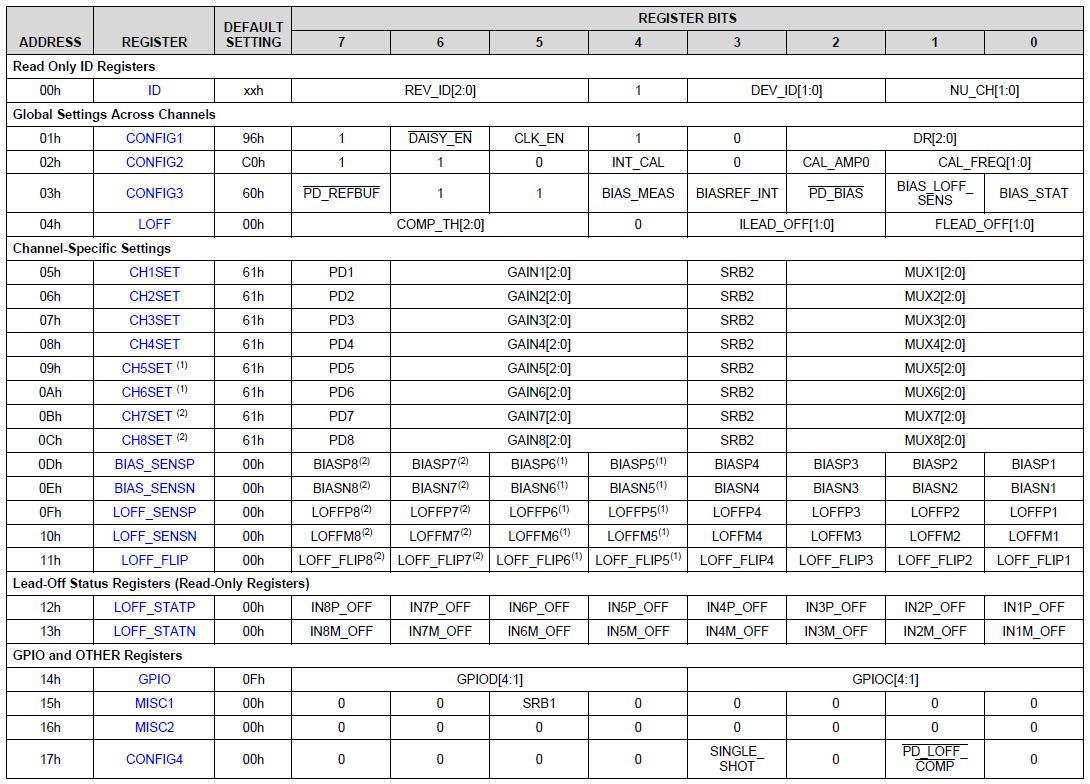
\includegraphics[width=\textwidth]{Tabla_registros_ADS}
    \caption{Tabla de registros de la familia ADS}
    \label{tab:Conf_Reg_ADS}
\end{table}

Una descripción más detallada de cada uno de los bits de cada registro se puede encontrar en el \textit{datasheet} del componente\cite{Datasheet_ADS}.

Como se puede ver en la tabla \ref{tab:Conf_Reg_ADS}, los convertidores cuentan con una gran cantidad de opciones de configuración. Para el desarrollo de este proyecto se ha implementado un sistema de configuración que permite la lectura y escritura de todos los registros.

\subsection{Transmisión de datos\label{sec:Transmisión_N}}

Tras completar el proceso de adquisición de datos resulta necesario transmitir dicha información hacia un dispositivo capaz de procesarla. Para ello la placa original contaba con dos alternativas. La primera consiste en, mediante \acrshort{USB} y acopladores aislantes, transmitir la información a un ordenador. 
\\La segunda hace uso de dos tecnologías inalámbricas distintas que funcionan de forma excluyente y son seleccionables con un \textit{jumper}: WiFi o Bluetooth.

\subsubsection{WiFi\label{sec:WiFi_N}}

Para la transmisión de datos a través de WiFi se seleccionó el módulo ESP12-E, basado en el \acrshort{SoC} ESP2866, también conocido nodemcu.
\\Este cuenta con un microcontrolador (\acrshort{MCU}) embebido de 32 bits (Tensilica L106) con una memoria \acrshort{RAM} de 36kB y una velocidad de reloj de la \acrshort{CPU} de hasta 80MHz, proporcionando suficiente potencia para las tareas básicas.

Así mismo se incluye montado en el mismo paquete una memoria flash de 4MB en la que almacenar el código de los programas que se ejecutarán y una antena embebida, dotando al módulo de conectividad en la banda de 2.4GHz.

\begin{figure} [h]
    \centering
    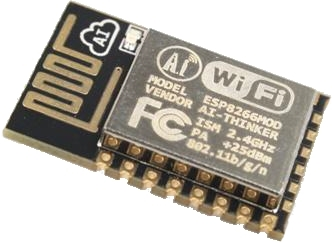
\includegraphics[width=6cm]{ESP8266}
    \caption{ESP8266}
    \label{fig:ESP8266}
\end{figure}

A efectos de diseño es muy importante saber cuales serán las entradas/salidas del dispositivo así como los pines dedicados para su programación. La figura \ref{fig:ESP8266_pinout} muestra un resumen de todas las funciones de cada uno de los pines. Como se puede observar, el \acrshort{SPI} hace uso de los pines 5, 6, 7 y 16. Por otro lado el \acrshort{UART}, necesario para la programación del micro hace uso de los pines 16 y 17. Dichos pines deberán reservarse posteriormente en la fase de diseño de la \acrshort{PCB}.

El dispositivo tiene tres modos de arranque dependiendo del sitio desde el que cargue el código y la selección de uno u otro modo viene determinada por los pines MTDO, GPIO0 y GPIO2. \\La tabla \ref{tab:ESP_Boot_Modes} resume los distintos modos de arranque así como el estado en el que debe estar cada uno de los pines para entrar en ese modo.
\begin{table} [h]
 	\centering
	\begin{tabular}{|c|c|c|c|c|}
		\hline 
		MTDO & GPIO0 & GPIO2 & Modo & Descripción \\ 
		\hline 
		L & L & H & UART & Descarga el código desde UART \\ 
		\hline 
		L & H & H & Flash & Carga desde memoria Flash a través de SPI \\ 
		\hline 
		H & x & x & SDIO & Carga desde una tarjeta SD \\ 
		\hline 
	\end{tabular} 
	\caption{Modos de arranque del ESP12-E\cite{ESP_Boot_mode}}
    \label{tab:ESP_Boot_Modes}
\end{table}	

\clearpage

\begin{figure} [h]
    \centering
    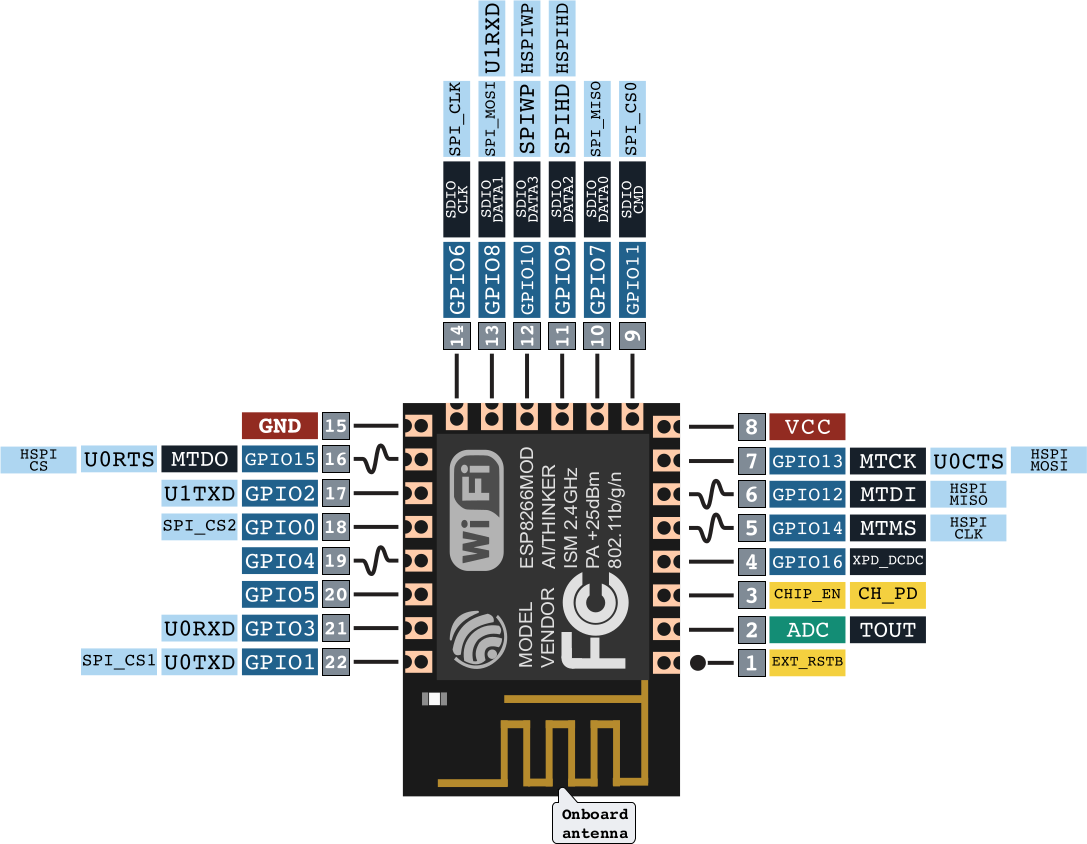
\includegraphics[width=\textwidth]{esp8266-esp12e-pinout}
    \caption{Resumen de todas las Entradas/Salidas del ESP12-E\cite{ESP_Pinout}}
    \label{fig:ESP8266_pinout}
\end{figure}

\subsubsection{Bluetooth\label{sec:Bluetooth_N}}

Para la transmisión de datos a través de Bluetooth se seleccionó el módulo Simblee™ RFD77101 ya que al igual que el módulo WiFi, cuenta con interfaces de comunicación a través de \acrshort{SPI} para conectarse con el \acrshort{ADC} (pines 21, 22, 31 y 32) y de \acrshort{UART} para su programación posterior programación (pines 23 y 24).

\begin{figure} [H]
    \centering
    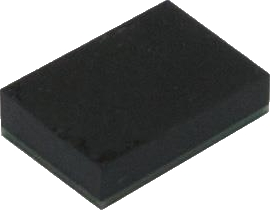
\includegraphics[width=5cm]{BT}
    \caption{Simblee™ RFD77101}
    \label{fig:BT}
\end{figure}

El módulo presenta un ARM Cortex-M0 como \acrshort{CPU} con 128KB de memoria Flash, 24KB de \acrshort{RAM} y una frecuencia de reloj de 16MHz. 

Todos los dispositivos de transmisión inalámbrica anteriormente mencionados permiten su programación utilizando el \acrshort{IDE} de Arduino lo cual facilita sensiblemente el proceso de desarrollo y prototipado teniendo la ventaja adicional de que es Software Libre.


\subsubsection{USB\label{sec:USB_N}}


Como este proyecto tiene como objetivo independizar el sistema lo máximo posible del ordenador se ha optado por desestimar el sistema de transmisión por \acrshort{USB} conservando solamente la interfaz inalámbrica. 

\section{Diseño final\label{sec:Diseño_final}}
          
Llegados a este punto se han analizado las características más importantes de cada uno de los elementos presentes en el sistema original, siendo los más importantes las distintas interfaces de comunicación y los pines de programación.
\\Con esta información ya es posible independizar cada uno de esos elementos y crear un nuevo diseño que cumpla con las especificaciones de este nuevo proyecto.

\begin{figure} [h]
    \centering
    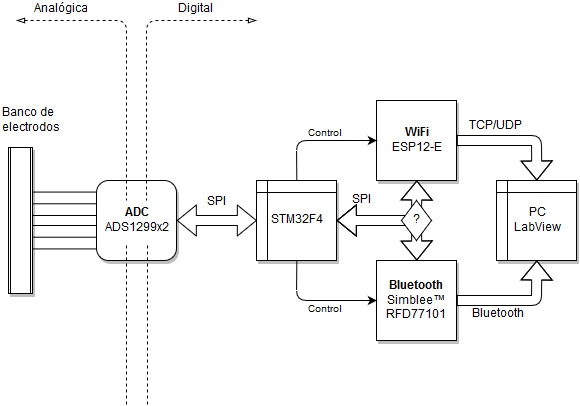
\includegraphics[width=12cm]{Esquema_proyecto_Javier}
    \caption{Esquema del proyecto final}
    \label{fig:Esquema_proyecto_Javier}
\end{figure}

El nuevo sistema estará compuesto por tres partes:
\begin{itemize}
\item En primer lugar etapa de adquisición compuesta de un banco de electrodos con sus correspondientes filtros analógicos y dos \acrshort{ADC}. 
\item Posteriormente un microcontrolador se encargará de realizar el procesado de la señal y la gestión de los distintos elementos.
\item Por último la transmisión de datos se realizará de forma inalámbrica a un ordenador u otro dispositivo mediante Bluetooth o WiFi.
\end{itemize}

Como se puede observar en la figura \ref{fig:Esquema_proyecto_Javier}, el ordenador sigue estando presente en el sistema pero en esta ocasión su función se limita a mostrar la información siendo fácilmente sustituible en un futuro por un dispositivo menos potente y barato. Al utilizar un microcontrolador en la propia placa de adquisición se consigue aumentar la independencia del sistema y se dota de unas características muy interesantes, tanto de procesado de señal como de almacenaje de la misma o gestión del consumo.

\subsection{Selección del microcontrolador\label{sec:Sel_micro}}

El microcontrolador es el núcleo del sistema. Para poder interactuar con todos los elementos anteriormente descritos deberá contar con las siguientes características:
\begin{itemize}
\item Bajo precio.
\item Bajo consumo.
\item Capacidad procesado de señal.
\item Para poder utilizar el máximo de la velocidad de adquisición de los ADS (16k\acrshort{SPS}) y evitar cuellos de botella, deberá contar con un Bus SPI de al menos 5.85Mb/s dedicados para la transmisión y la misma cantidad para recepción o dos buses.
\[Tasa\ de\ transferencia = 16k\ Muestras/s * 8\ canales * 24bits * 2\ ADS = 5.85Mb/s\]

\end{itemize}

Hay una gran cantidad de microcontroladores en el mercado que podrían utilizarse para este proyecto pero, de entre todos los disponibles, aquellos con arquitectura \textbf{ARM} son los que mejor se adaptan a las especificaciones. Concretamente los más adecuados son aquellos englobados en la familia \textbf{Cortex M4} ya que están especialmente diseñados con \acrshort{DSP} integrado para conseguir un rendimiento máximo minimizando el consumo.

\begin{figure}[h]
  \begin{subfigure}[b]{0.49\textwidth}
   	\centering
    
\includegraphics [height=2.5cm]{Texas_Instument}
    \caption{Logo de Texas Instument}
    \label{fig:Logo_TI}
  \end{subfigure}
  \hfill
  \begin{subfigure}[b]{0.49\textwidth}
  	\centering
    
\includegraphics[height=2.5cm]{STMicroelectronics}
    \caption{Logo de STMicroelectronics}
    \label{fig:Logo_STM}
  \end{subfigure}
  \caption{Principales fabricantes contemplados}
\end{figure}

\clearpage

La tabla \ref{tab:Comparativa_MCU} muestra varios dispositivos de esa familia vendidos por Texas Instrument o STMicroelectronics y un resumen de sus características principales.
\begin{table} [h]
	\centering
	\begin{tabular}{|c|c|c|c|c|}
\hline 
 &\multicolumn{2}{c|}{Texas Instruments}& \multicolumn{2}{c|}{STMicroelectronics} \\ 
\hline 
 & TM4C123GH6PM & TM4C1294NCPDT & STM32F405& STM32F469  \\ 
\hline 
\acrshort{FCPU} [MHz] & 80 & 120 & 168 & 180 \\ 
\hline 
Flash [kB] & 256 & 1024 & 1024 & 2048 \\ 
\hline 
\acrshort{RAM} [kB] & 32 & 256 & 192 & 384 \\ 
\hline 
\acrshort{SPI} & x4 & x4 & x2 + 1 & x6 \\ 
\hline 
Precio [€] & 8,72 & 12,74 & 9,24 & 13,48 \\ 
\hline 
	\end{tabular} 
	\caption{Comparativa entre distintos MCUs}
	\label{tab:Comparativa_MCU}
\end{table}

Todos los dispositivos anteriormente contemplados tienen \acrshort{DSP} integrados así como una Unidad de Punto Flotante (\acrshort{FPU}) que permite realizar operaciones matemáticas avanzadas de forma óptima.

Entre los dispositivos anteriores, los pertenecientes a la familia STM presentan mejor relación coste/prestaciones, pero el verdadero factor diferenciador son las herramientas dispuestas para la comunidad por parte del fabricante.
\\En la página web se pueden encontrar distintas herramientas y PDFs que facilitan sensiblemente el proceso de desarrollo para esta plataforma. 

Finalmente se seleccionó el \acrshort{MCU} STM32F405 en el formato \acrshort{LQFP64} ya que sus características se ajustan perfectamente a las especificaciones, manteniendo unas muy buenas prestaciones y un precio bastante bajo. Todo esto con el valor añadido de que ya se contaba con la placa de desarrollo STM32F4 Discovery lo cual permitió comenzar con el aprendizaje y estudio del entorno sin la necesidad de esperar al diseño, impresión y soldado de la placa final.

\begin{figure} [h]
    \centering
    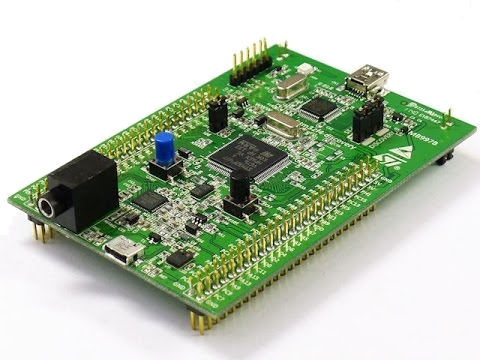
\includegraphics[width=5cm]{STM32F4_Discovery}
    \caption{Placa de desarrollo STM32F4 Discovery}
    \label{fig:STM32F4_Discovery}
\end{figure}

El \acrshort{MCU} cuenta con 3 buses SPI independientes que pueden funcionar en modo \textit{\gls{Full Duplex}}. El SPI$_1$  es capaz de funcionar hasta 42Mb/s mientras que los SPI$_2$ y SPI$_3$ pueden comunicar información hasta 21Mb/s. Los pines dedicados a dichos buses se pueden consultar en el \textit{Datasheet} del componente\cite{Datasheet_STM}.
\\Otra característica interesante de este \acrshort{MCU} es la presencia de forma nativa de un gestor de \acrshort{USB} \acrlong{OTG} (\acrshort{OTG}) permitiendo así conectar un dispositivo \acrshort{USB} para almacenar información a largo plazo.

\clearpage

\subsection{Alimentación\label{sec:Alimentación}}

Tras seleccionar todos los elementos se va a proceder a escoger una alimentación que permita a todos los dispositivos funcionar en condiciones óptimas.
\\La tabla \ref{tab:Alimentacion} muestra un resumen de todos los elementos presentes en el sistema junto con los rangos de voltaje recomendados por los fabricantes para su alimentación.

\begin{table} [h]
	\centering
	\begin{tabular}{|c|c|c|}
	\hline 
	Dispositivo & V$_{min}$ [V] & V$_{max}$ [V] \\ 
	\hline 
	Simblee BT & 1.8 & 3.6 \\ 
	\hline 
	ESP12-E & 3.0 & 3.6 \\ 
	\hline 
	STM & 1.8 & 3.6 \\ 
	\hline 
	ADS (Digital) & 1.8 & 3.6 \\ 
	\hline 
	ADS (Analógica) & 4.75 & 5.25 \\ 
	\hline 
	USB & 5 & 5 \\ 
	\hline 
	\end{tabular} 
	\caption{Rangos de alimentación de todos los elementos}
	\label{tab:Alimentacion}
\end{table}

De la tabla \ref{tab:Alimentacion} se deduce que para que todos los dispositivos funcionen correctamente será necesario dotar a la placa de 5 voltios con los que se podrá alimentar la parte analógica del ADS así como el USB mientras que la parte digital se puede alimentar en el rango de 3V a 3.6V. 

Por motivos de compatibilidad con el diseño anterior y tras comprobar que se cumple con los requisitos impuestos por los nuevos elementos del sistema se ha optado por mantener el mismo esquema de alimentación que en el proyecto base.

El sistema de alimentación se compone de dos partes principales, cada una encargada de proporcionar el voltaje deseado manteniendo el ruido generado por el mismo al mínimo.

\subsubsection{Alimentación 3.3V\label{sec:Alimentacion_3.3V}}
Para conseguir un voltaje de 3.3V estable se ha utilizado el regulador AZ1117C-3.3 ya que es capaz de conseguir una precisión para el voltaje de salida del $\pm$1\% así como un ruido de salida de 0.003\% V$_{out}$ entre 10Hz y 10kHz.
En la figura \ref{fig:Alim_3.3} se muestra el esquema eléctrico utilizado, que es una variación del circuito recomendado por el fabricante en su \textit{datasheet}\cite{Datasheet_3.3}.

\begin{figure} [h]
    \centering
    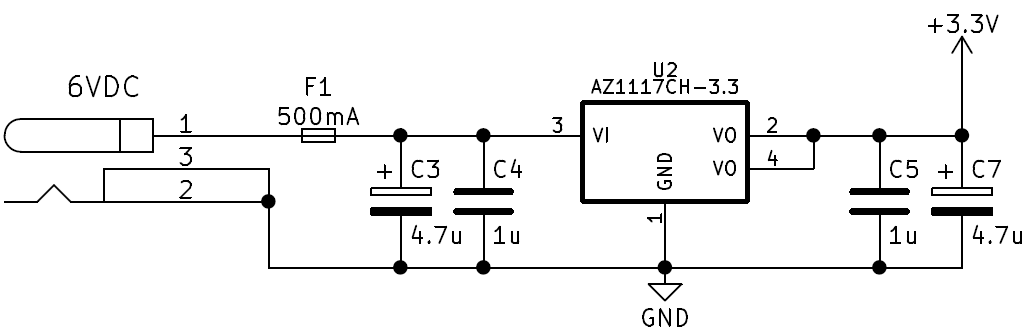
\includegraphics[width=10cm]{Alim_3_3}
    \caption{Esquema de alimentación a 3.3V}
    \label{fig:Alim_3.3}
\end{figure}

\subsubsection{Alimentación 5V\label{sec:Alimentacion_5V}}

Los 5V serán utilizados por el dispositivo de almacenamiento USB para su alimentación y por el ADS para generar los distintos voltajes de referencia que necesita para operar correctamente. Al afectar de forma directa a las mediciones realizadas por el ADS la eliminación de variaciones en este voltaje es crucial, pues estas supondrán un ruido añadido a la señal final.

El regulador encargado de proporcionar 5V es el MCP1711. Este integrado está caracterizado por tener un rizado de salida menor al 1\% del voltaje de salida así como de poseer una corriente en reposo muy baja. Este último parámetro facilitará el diseño de un sistema portátil alimentado por baterías aumentando la duración de la misma. La figura \ref{fig:Alim_5} muestra el esquema eléctrico utilizado.

\begin{figure} [h]
    \centering
    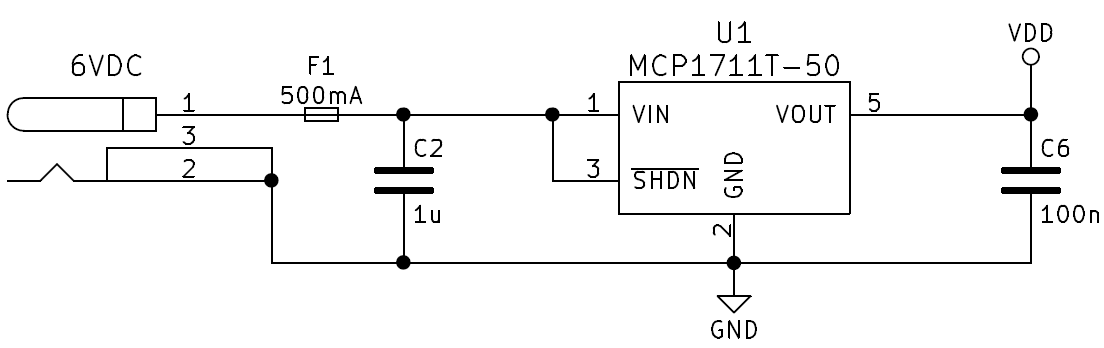
\includegraphics[width=10cm]{Alim_5}
    \caption{Esquema de alimentación a 5V}
    \label{fig:Alim_5}
\end{figure}

Para funcionar correctamente ambos integrados necesitan que el voltaje de entrada sea superior al voltaje de salida en un factor que en la documentación técnica recibe el nombre de ``\gls{Tensión de Dropout}''(V$_{DROP}$).
\\De acuerdo al Datasheet de ambos reguladores, V$_{DROP}$ es para 3.3V y 5V, 1.3V y 0.43V respectivamente. Con esa información se deduce que el integrado que limita el diseño es el regulador de 5V así como que con una entrada de al menos 5.43V ambos reguladores deberían funcionar correctamente.

Finalmente se ha optado por una fuente de alimentación de 6V ya que esto permitirá hacer uso de pilas o baterías para alimentar el sistema, dotándolo de independencia de la red eléctrica y eliminando el riesgo de electrocución.

\clearpage

\section{Circuito electrónico y esquemáticos\label{sec:Esquemáticos}}

El último paso de la fase de desarrollo será generar un esquemático capaz de englobar todos los elementos anteriormente presentados, interconectarlos y dar como resultado un sistema funcional.

En este punto es importante valorar dos alternativas de diseño, cada una con sus ventajas e inconvenientes: Implementación de todo el circuito de cero o crear una placa que se conecte a la ya existente.

Si bien es cierto que para un diseño final crear una placa que englobe todos los componentes sería lo ideal, pues presentaría un formato más compacto y mejor presentación, hacerlo también supone crear una placa más grande y desaprovechar aquellas ya construidas en proyectos anteriores.

Teniendo en cuenta que se cuenta con varias placas ya montadas y que el sistema está en fase de prototipo, se va a optar por la segunda opción, creando una segunda placa independiente en la que se incluirán todos los elementos correspondientes a la gestión de las señales digitales del sistema, dejando las señales analógicas en la otra placa. De esta forma la fase de diseño de la \acrshort{PCB} y de montaje se simplifica considerablemente y se abaratan costes al reutilizarse componentes.

Para la conexión con la otra placa se aprovechará el espacio dejado por el módulo ESP12-E, pues al hacer uso de \acrshort{SPI} es posible obtener todas las señales necesarias para interactuar con el ADS.

El sistema embebido en esta placa incluirá los elementos que se pueden ver en la figura \ref{fig:Esquematico_global}

\begin{figure} [h]
    \centering
    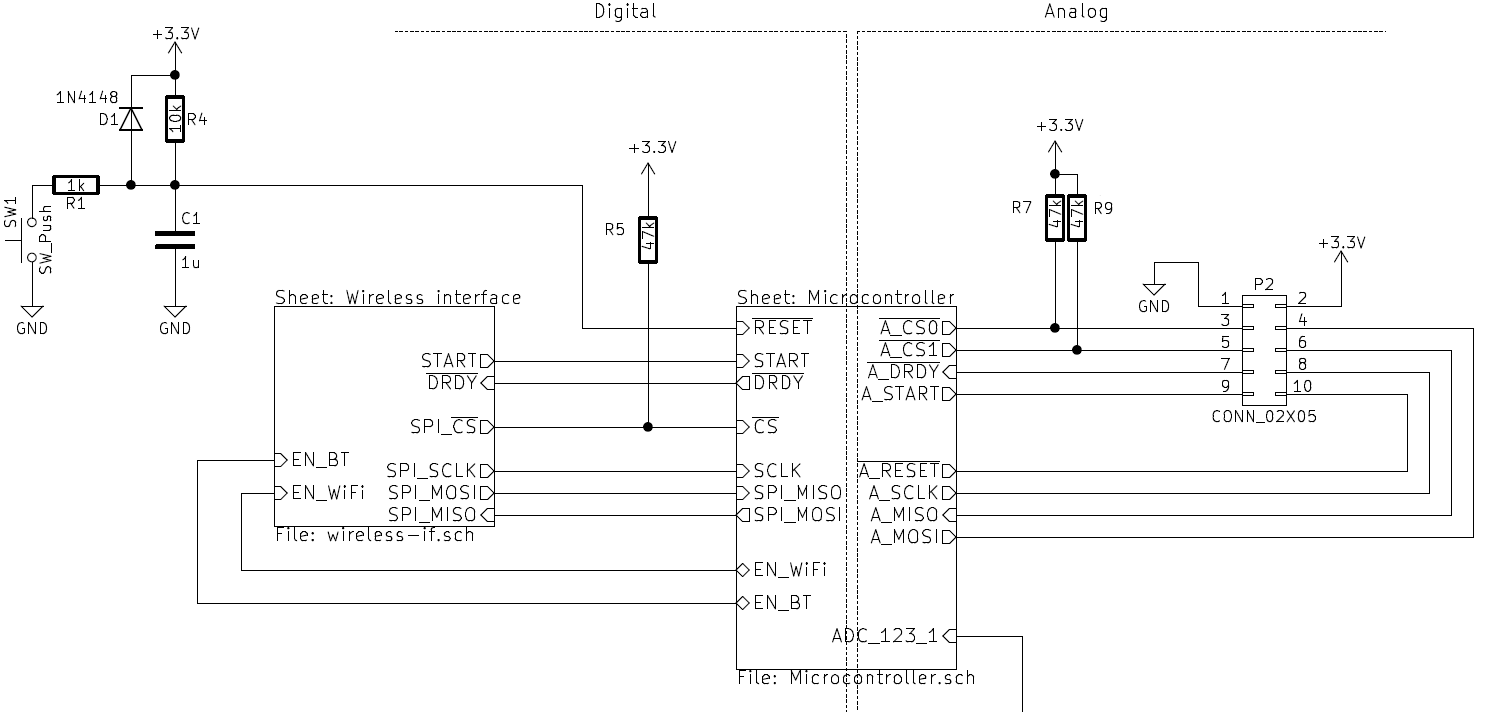
\includegraphics[width=14cm]{Esquematico_global}
    \caption{Esquema general del sistema}
    \label{fig:Esquematico_global}
\end{figure}

Se ha incluido en la placa un botón de reinicio con su correspondiente circuito electrónico así como una realimentación desde la alimentación hasta uno de los pines \acrshort{ADC} el microcontrolador para poder monitorizar el estado de la batería.

\subsection{Circuito de alimentación\label{sec:Esquemáticos_alim}}

Aunando los dos circuitos presentados en la sección \ref{sec:Alimentación} el resultado final es el obtenido en la figura \ref{fig:Alim_final}.

\begin{figure} [h]
    \centering
    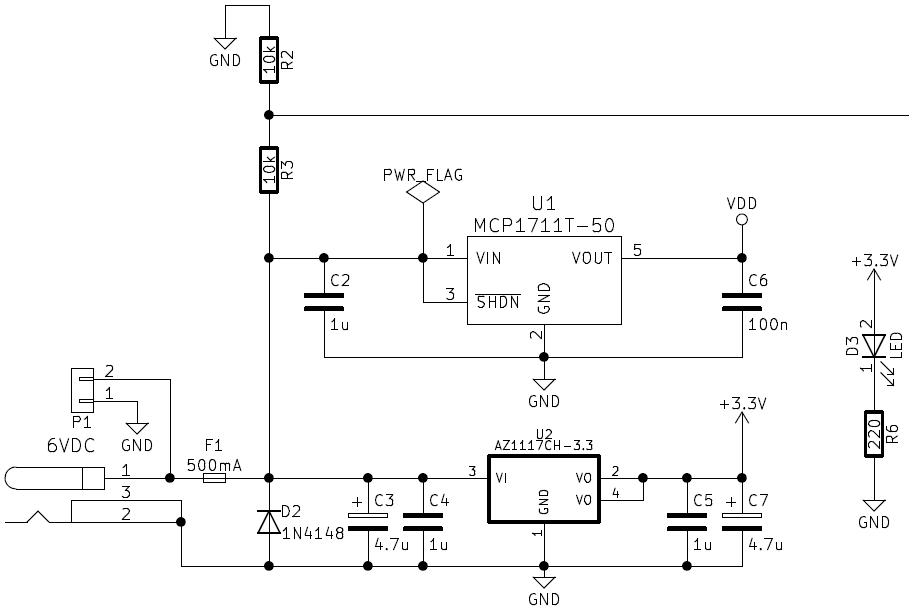
\includegraphics[width=14cm]{Alim_final}
    \caption{Esquemático final del circuito de alimentación}
    \label{fig:Alim_final}
\end{figure}

El fusible (F1) garantiza que la máxima corriente que consumirá el dispositivo es de 500mA, evitando así que el sistema o el paciente sufran daños en caso de un cortocircuito. Adicionalmente se ha incluido un diodo \acrshort{LED} cuya función es indicar el estado de la placa. Si la placa ha encendido correctamente o si se encuentra en funcionamiento el \acrshort{LED} se encenderá.

El diodo (D2) junto con el condensador (C3) evitarán que los transitorios afecten al voltaje de entrada asegurando así que la alimentación que recibirán ambos integrados será lo más estable posible.

Con el objetivo de monitorizar el estado de la batería se ha utilizado el \acrshort{ADC} incorporado en el propio microcontrolador. Como la señal de entrada se encuentra fuera del rango soportado en las especificaciones del STM se ha optado por incorporar las resistencias R2 y R3 formando un divisor de tensión utilizando así la señal resultante para realizar las medidas.

\clearpage

\subsection{Microcontrolador\label{sec:Esquemáticos_micro}}

El microcontrolador es el núcleo del sistema. Este hace de centro de control de todas las señales digitales que se transmiten así como de gestor de dispositivos, decidiendo que dispositivos se encuentran activos en cada momento. 
Para gestionar que dispositivos se encuentran habilitados se ha sustituido el \textit{jumper} de la placa original por \acrshort{GPIO} del microcontrolador. De esta forma se consigue mayor flexibilidad, automatización y se optimiza el consumo. 

Adicionalmente se ha integrado un \acrshort{LED} conectado al pin PA9 que dotará a la placa de indicadores visuales del estado en el que se encuentra.

La figura \ref{fig:Esquematico_micro} muestra una representación del integrado así como todos los elementos con los que está conectado.

\begin{figure} [h]
    \centering
    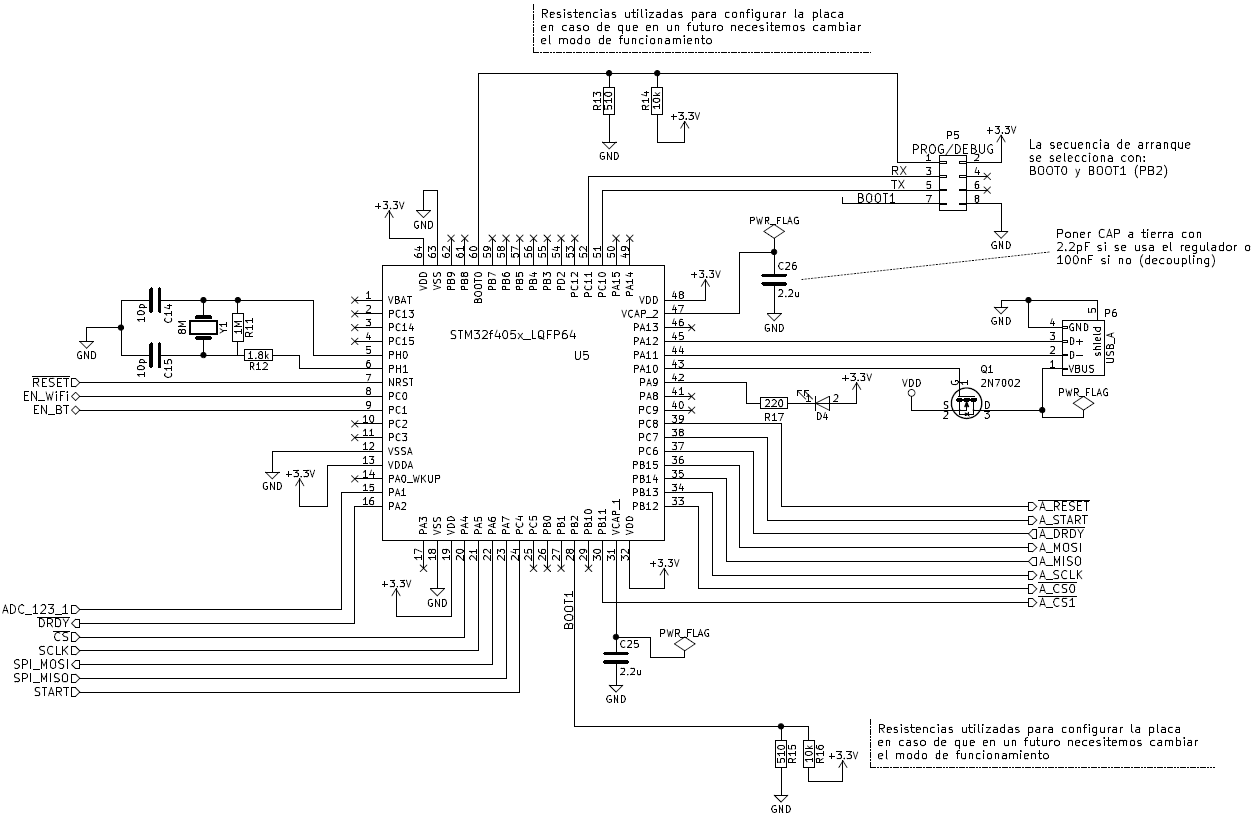
\includegraphics[width=\textwidth]{Esquematico_micro}
    \caption{Esquemático del microcontrolador}
    \label{fig:Esquematico_micro}
\end{figure}

El modo de arranque del dispositivo viene determinado por el estado de los pines Boot0 y Boot1. Haciendo uso de las resistencias R13, R14, R15 y R16 se consigue forzar que en condiciones normales de operación el STM arranque desde la memoria Flash integrada. 
\\Con el objetivo de reprogramar el microcontrolador se ha añadido el conector P5. Dicho conector permite alternar entre los distintos modos de arranque del STM así como interactuar con el por UART. Esta última característica será la que permitirá subir el código a ejecutar pero también brinda funciones de \textit{debug}.

\clearpage

El sistema aprovecha dos de los 3 buses \acrshort{SPI}. El bus SPI1, capaz de transmitir a 41Mb/s se ha reservado para la comunicación ESP12-E $\Longleftrightarrow$ STM32F4 mientras que el utilizado para comunicarse con los ADS es el SPI2 con una velocidad de hasta 21Mb/s.

El \acrshort{MCU} puede trabajar con un oscilador interno sin problemas pero la presencia de un oscilador externo basado en un cristal de cuarzo proporciona ciertas ventajas como son mayor precisión en el reloj y la posibilidad de usar \acrshort{PLL} para aumentar la frecuencia de trabajo del procesador.
\\El circuito asociado al cristal se puede observar en la parte superior izquierda de la figura \ref{fig:Esquematico_micro} pero se incluye a continuación para facilitar la lectura de este documento:

\begin{figure} [h]
    \centering
    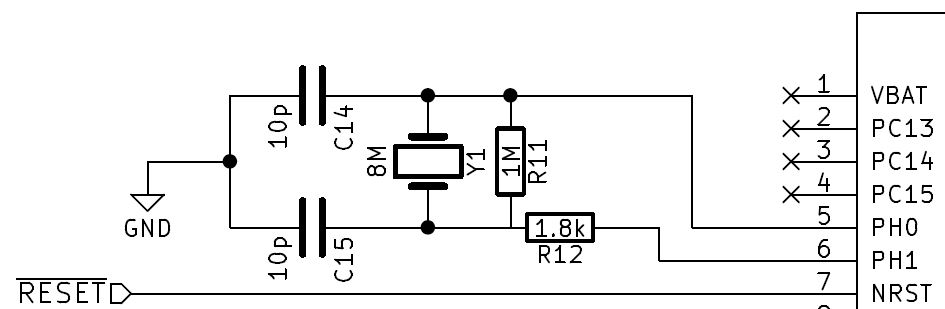
\includegraphics[width=10cm]{Detalle_cristal}
    \caption{Detalle del circuito asociado al oscilador externo}
    \label{fig:Detalle_cristal}
\end{figure}


Para realizar un diseño funcional del circuito del oscilador se ha utilizado el \textit{datasheet} del dispositivo junto con una guía de buenas prácticas\cite{Guia_Oscilador}, ambos proporcionados por el fabricante. La configuración utilizada a nivel de software para la gestión de dicho reloj se explicará en mayor profundidad en el capítulo \ref{sec:Implementacion}.

Se han añadido todos los condensadores recomendados por el fabricante. Algunos deben tener una capacidad determinada en función del modo de funcionamiento del microcontrolador (C25 y C26), otros, denominados condensadores de desacoplo, tienen como objetivo eliminar el ruido de altas frecuencias de la zona de alimentación. El condensador C11 es denominado Bulk y tiene como objetivo garantizar una alimentación lo más estable posible.

\begin{figure} [h]
    \centering
    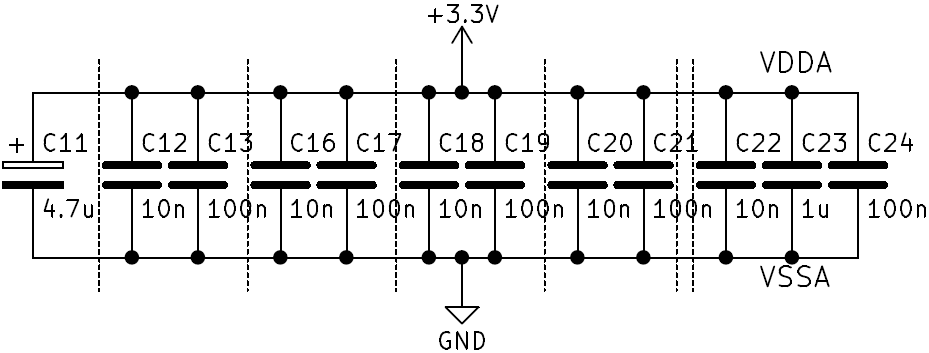
\includegraphics[width=10cm]{Condensadores_micro}
    \caption{Condensadores Bulk (C11) y de desacoplo}
    \label{fig:Condensadores_micro}
\end{figure}

 Por simplicidad y legibilidad se han agrupado todos en una zona del esquemático pero a la hora de diseñar la PCB será necesario tener presente que para que el dispositivo funcione correctamente estos últimos deben localizarse lo más cerca posible de los pines de alimentación.

Finalmente, como el \acrshort{MCU} tiene la capacidad de interactuar directamente con dispositivos \acrshort{USB}, con el objetivo de implementar en un futuro características que aprovechen dicha capacidad se ha añadido un conector \acrshort{USB} cuyo bus de alimentación se encuentra controlado por el propio \acrshort{MCU}. De esta forma es posible habilitar y deshabilitar el dispositivo USB y reducir el consumo.



%
% Implementación
%
\chapter{Implementación\label{sec:Implementacion}}

TODO: Implementación

Hardware
	PCB (Añadir BOM)
	
	Primeras pruebas y programación
	

Software
	Comunicación ADS - STM
	
	Comunicación STM- ESP
	
	Arduino (Comunicación ESP - PC)
	
	

%
% Resultados
%
\chapter{Resultados\label{sec:Resultados}}

TODO: Resultados

Gráficas, lecturas...

%
% Conclusiones
%
\chapter{Conclusiones\label{sec:conclusiones}}

TODO: Conclusiones sobre el trabajo realizado

Valoración del trabajo. Partes positivas, negativas y posibles mejoras. 

%
% Glosario
%
\printglossary[title=Glosario,toctitle=Glosario]
\printglossary[title=Acrónimos,toctitle=Acrónimos,type=\acronymtype]
%
% Página en blanco
%
\cleardoublepage

%
% Bibliografía
%
%\include{src/Bibliografia}
\nocite{*}
\printbibliography[heading=bibintoc]

% No expandir elementos para llenar toda la página
\raggedbottom

%
% Apéndices
%
\appendix
\cleardoublepage
\addappheadtotoc
\appendixpage

%
% TODO: Apéndices del TFM
%
\chapter{Ejemplos de bloques y comandos útiles en LaTeX\label{sec:ejemplos}}
\section{Ejemplo de sección}

%
% Breve guía de comandos útiles para la memoria
%

% Citar una referencia
%La DARPA creó el protocolo de Internet \cite{ipv4sta}.

% Citar un elemento del glosario
Citamos el acrónimo \gls{PCB}.

% Citar un elemento del glosario (primera letra en may´usculas)
\Gls{bitstream} es una secuencia de bits.

% Insertar una imagen con pie de página
\begin{figure}[htp!]
  \centering
  
\includegraphics[width=0.75\textwidth,clip=true]{logo_politecnica}
  \caption{Logo de la Universidad Politécnica de madrid.}
  \label{fig:logo_uam}
\end{figure} 

% Referenciar una etiqueta (label)
La figura~\ref{fig:logo_uam} se utiliza en la portada.

% Nueva página
\clearpage

% Añadir código fuente sin líneas
\begin{lstlisting}[label=algoritmo:quicksort,language=C,frame=single,caption=Algoritmo de ordenación Quicksort]
#include <stdio.h>
 
void quick_sort (int *a, int n) {
    int i, j, p, t;
    if (n < 2)
        return;
    p = a[n / 2];
    for (i = 0, j = n - 1;; i++, j--) {
        while (a[i] < p)
            i++;
        while (p < a[j])
            j--;
        if (i >= j)
            break;
        t = a[i];
        a[i] = a[j];
        a[j] = t;
    }
    quick_sort(a, i);
    quick_sort(a + i, n - i);
}
\end{lstlisting}

% Bloque de código inseparable
\begin{code}
#include <stdio.h>
 
void quick_sort (int *a, int n) {
    int i, j, p, t;
    if (n < 2)
        return;
    p = a[n / 2];
    for (i = 0, j = n - 1;; i++, j--) {
        while (a[i] < p)
            i++;
        while (p < a[j])
            j--;
        if (i >= j)
            break;
        t = a[i];
        a[i] = a[j];
        a[j] = t;
    }
    quick_sort(a, i);
    quick_sort(a + i, n - i);
}
\end{code}

% Fórmula dentro de una línea de texto
La ecuación de Euler ($e^{ \pm i\theta } = \cos \theta \pm i\sin \theta$) es citada frecuentemente como un ejemplo de belleza matemática.

% Fórmula independiente
\begin{equation}\label{eq:pythagoras}
a^2 + b^2 = c^2
\end{equation}


\begin{lstlisting}[language=Python, caption=Python example]
import numpy as np
    
def incmatrix(genl1,genl2):
    m = len(genl1)
    n = len(genl2)
    M = None #to become the incidence matrix
    VT = np.zeros((n*m,1), int)  #dummy variable
    
    #compute the bitwise xor matrix
    M1 = bitxormatrix(genl1)
    M2 = np.triu(bitxormatrix(genl2),1) 

    for i in range(m-1):
        for j in range(i+1, m):
            [r,c] = np.where(M2 == M1[i,j])
            for k in range(len(r)):
                VT[(i)*n + r[k]] = 1;
                VT[(i)*n + c[k]] = 1;
                VT[(j)*n + r[k]] = 1;
                VT[(j)*n + c[k]] = 1;
                
                if M is None:
                    M = np.copy(VT)
                else:
                    M = np.concatenate((M, VT), 1)
                
                VT = np.zeros((n*m,1), int)
\end{lstlisting}

\lstlistoflistings


%AÑADIR DE ANEXO EL BOM

% Fin del documento
\end{document}
